\documentclass[12pt]{article}
\usepackage[backend=biber, style=alphabetic, sorting=ynt]{biblatex}
\usepackage[utf8]{inputenc} % Datei ist in UTF-8 encoded 
\usepackage[T1]{fontenc}   % font encoding
\usepackage{courier} % courier font, usage: \texttt{This is Courier font.}
\usepackage[german]{babel} % deutsche Umlaute
\usepackage{csquotes}
\usepackage{epigraph}  % ein epigraph ist ein schönes Zitat am Anfang
\usepackage{graphicx} % Required to insert images
\usepackage{mathtools} % absmath with benefits
\usepackage{listings} % source code listings
\usepackage{authblk} % multiple authors
\usepackage{xcolor} % colored things

\usepackage{fancyhdr} % Required for custom headers
\usepackage{extramarks} % Required for headers and footers

\usepackage{booktabs} % neat table formatting
\usepackage{longtable} % tables over more than one page
\renewcommand{\arraystretch}{1.2} % mehr Zeilenabstand bei Tabellen
\setlength\heavyrulewidth{0.25ex} % thicker top and bottom lines in tables
\newcommand{\tabitem}{~~\llap{\textbullet}~~} % use items in tables with \tabitem XXX
\usepackage[labelfont=bf]{caption} % captions for tables without float
\captionsetup[table]{justification=raggedright,singlelinecheck=false} % tables have left aligned captions
\usepackage{xparse}

\usepackage[bookmarks=true]{hyperref}
\usepackage{glossaries}

\makeglossaries

\newsavebox{\fminipagebox}
\NewDocumentEnvironment{framedminipage}{m O{\fboxsep}}
 {\par\kern#2\noindent\begin{lrbox}{\fminipagebox}
  \begin{minipage}{#1}\ignorespaces}
 {\end{minipage}\end{lrbox}%
  \makebox[#1]{%
    \kern\dimexpr-\fboxsep-\fboxrule\relax
    \fbox{\usebox{\fminipagebox}}%
    \kern\dimexpr-\fboxsep-\fboxrule\relax
  }\par\kern#2
 }

\addbibresource{Quellen.bib}

% Standard-Schriftart
\renewcommand{\familydefault}{\sfdefault}
\usepackage{helvet}

% Margins
\topmargin=-0.45in
\evensidemargin=0in
\oddsidemargin=0in
\textwidth=6.5in
\textheight=9.0in
\headsep=0.25in
\linespread{1.1} % Line spacing
\setlength\parindent{0pt} % Removes all indentation from paragraphs

% Nummerierung
\setcounter{secnumdepth}{4} % Tiefe in der Überschriften-Nummerierung endet
\setcounter{tocdepth}{3} % Tiefe des Inhaltsverzeichnisses

% Set up the header and footer
\pagestyle{fancy}
\lhead{} % Top left header
\chead{} % Top center head
\rhead{\leftmark} % Top right header
\lfoot{} % Bottom left footer
\rfoot{\thepage} % Bottom center footer
\cfoot{} % Bottom right footer
\setlength{\headheight}{15.5pt}
\renewcommand\headrulewidth{0.4pt} % Size of the header rule
\renewcommand\footrulewidth{0.4pt} % Size of the footer rule

%----------------------------------------------------------------------------------------
%	Codestyle section
%----------------------------------------------------------------------------------------
\lstset{basicstyle=\footnotesize\ttfamily,breaklines=true}

 \lstset{
         basicstyle=\footnotesize\ttfamily, % Standardschrift
         numberstyle=\tiny,          % Stil der Zeilennummern
         numbersep=5pt,              % Abstand der Nummern zum Text
         tabsize=2,                  % Groesse von Tabs
         extendedchars=true,         %
         breaklines=true,            % Zeilen werden Umgebrochen
         keywordstyle=\color{red},
            frame=b,         
         stringstyle=\color{white}\ttfamily, % Farbe der String
         showspaces=false,           % Leerzeichen anzeigen ?
         showtabs=false,             % Tabs anzeigen ?
         xleftmargin=17pt,
         framexleftmargin=17pt,
         framexrightmargin=5pt,
         framexbottommargin=4pt,
         showstringspaces=false      % Leerzeichen in Strings anzeigen ?        
 }
\lstloadlanguages{Java}
\usepackage{caption}
\DeclareCaptionFont{white}{\color{white}}
\DeclareCaptionFormat{listing}{\colorbox[cmyk]{0.43, 0.35, 0.35,0.01}{\parbox{\textwidth}{\hspace{15pt}#1#2#3}}}
\captionsetup[lstlisting]{format=listing,labelfont=white,textfont=white, singlelinecheck=false, margin=0pt, font={bf,footnotesize}}
\renewcommand{\lstlistingname}{Code} % "Code" statt "Listing"
\newcommand{\code}[1]{\texttt{#1}}   % \Code{if then else} für inline code

%----------------------------------------------------------------------------------------
%	NAME AND CLASS SECTION
%----------------------------------------------------------------------------------------

\newcommand{\Title}{Dokumentation Dateiserver-Gruppen 5 + 10} % Assignment title
\newcommand{\DueDate}{03.09.2016} % Due date
\newcommand{\Class}{Fachpraktikum IT-Sicherheit} % Course/class
\newcommand{\ClassTime}{} % Class/lecture time
\newcommand{\ClassInstructor}{Ralf Naues} % Teacher/lecturer

%----------------------------------------------------------------------------------------
%	TITLE PAGE
%----------------------------------------------------------------------------------------

\title{
\vspace{0.5in} %2in ohne Bild
\textmd{\textbf{\Class:\ \Title}}\\
\normalsize\vspace{0.1in}\small{Abzugeben\ am\ \DueDate}\\
\vspace{0.1in}\large{\textit{Betreuung durch \ClassInstructor\ \ClassTime}}
\vspace{1in} % 3in ohne Bild
}

\author[1]{Christoph Weißenborn}
\author[1]{Jörg Ricardo Schumacher}
\author[1]{Marc Ernst Eddy Woerkom}
\author[1]{Patrick Häbel}
\author[2]{Sascha Girrulat}
\author[2]{Silas Jansen}
\author[1]{Waldemar Schmidt}
\affil[1]{Gruppe 5 (Nord)}
\affil[2]{Gruppe 10 (Süd)}
\date{} % Insert date here if you want it to appear below your name


\begin{document}

\maketitle

\vfill
\begin{center}-
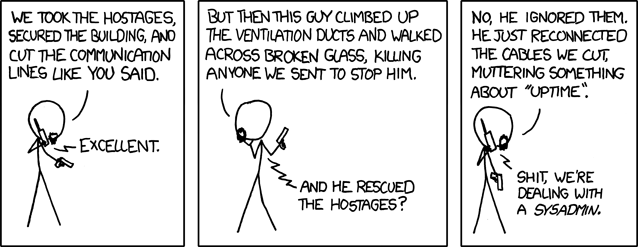
\includegraphics[scale=0.5]{images/0705.png}
\end{center}

%----------------------------------------------------------------------------------------
%	TABLE OF CONTENTS
%----------------------------------------------------------------------------------------

%\setcounter{tocdepth}{1} % Uncomment this line if you don't want subsections listed in the ToC

\newpage
\tableofcontents
\newpage

%----------------------------------------------------------------------------------------
%	ZUSAMMENFASSUNG
%----------------------------------------------------------------------------------------

\begin{abstract}
Unsere Aufgabe war die Bereitstellung zweier Dateiserver innerhalb der vorgegebenen VPN-Netzwerkumgebung. Dabei waren wir verantwortlich für Organisation, Kommunikation und Dokumentation des Projektes. Unser Projekt hatte kein Budget, keine zentrale Leitung und keine festen Arbeitszeiten. Das agile Verfahren Kanban mit einem Trello-Board hat uns daher sehr geholfen, unsere wichtigsten Ziele dennoch zeitgerecht zu erreichen.\\

Da das Projekt im Rahmen des Fachpraktikums IT-Sicherheit durchgeführt wurde, haben wir ein besonderes Augenmerk auf das Sicherheitskonzept gelegt; der BSI IT-Grundschutz diente uns als Maßstab für die Analyse der Sicherheitsanforderungen.\\

Bei der technischen Umsetzung hoffen wir, mit dem Konfigurationsmanagement-Werkzeug Ansible und einer zentralen Codeverwaltung mittels Github ein solides Fundament für eine mögliche Weiterverwendung der technischen Ergebnisse gelegt zu haben.\\

Es ist uns in der vorgegebenen Zeit gelungen, zwei Samba/SMB-Server für die Anwender zur Verfügung zu stellen und $95\%$ aller Sicherheits-Maßnahmen umzusetzen, die wir uns vorgenommen hatten. Alles was wir nicht umsetzen konnten -- meist weil uns Zeit, Geld oder Zuarbeit gefehlt haben -- ist nicht in Vergessenheit geraten: Im Ausblick haben wir geplante technische Maßnahmen und gewünschte organisatorische Regelungen aufgelistet.
\end{abstract}
%----------------------------------------------------------------------------------------
%	SECTION GRUNDLAGEN
%----------------------------------------------------------------------------------------

\newpage
\section{Grundlagen}

\setlength{\epigraphwidth}{.9\textwidth}
\epigraph{"`Tatsache ist, dass -- ohne begleitende Richtlinien oder einen Mechanismus zur Beurteilung -- Sicherheit von jedem anders definiert wird und von niemandem verifiziert werden kann. Es gibt keinen Maßstab für eine Übereinstimmung mit einer „Kultur“ und eine „Sicherheitskultur“ wird immer von einer Kultur „erledige die Arbeit“ außer Kraft gesetzt werden.\newline \\ Wenn es Regeln gibt, schreibe sie auf. Wenn Technologien genutzt werden, um die Regeln zu implementieren oder zu überwachen, dann schreibe auch das auf. Wenn Leute die Regeln brechen, lasse Konsequenzen folgen. Wenn die Regeln legitime Arbeiten verhindern, dann ändere sie. So einfach ist das."'}{\textit{übersetzt aus „Ten claims that scare security pros“, infoworld.com}}

Unsere Gruppen (5 und 10) haben den Auftrag erhalten, jeweils einen Datei-Server einzurichten und in Betrieb zu nehmen. Wir waren selbst dafür verantwortlich, das Projekt zu organisieren und die Zusammenarbeit mit den anderen Gruppen zu regeln, welche für Netz, CA, Mail und Webserver zuständig waren. Das Spannendste an diesem Projekt war für uns natürlich die Frage nach der IT Sicherheit. Sie steht im Spannungsfeld zwischen notwendiger ganzheitlicher Betrachtung des Themas und dem beschränkten Auftrag zwei Dateiserver bereit zu stellen.\\

Wo wir Risiken gefunden haben, die mit technischen Mitteln alleine nicht zu administrieren sind, haben wir organisatorische Regelungen geschaffen. Bei Risiken , welche wir alleine nicht absichern konnten, haben wir stets auf die Kommunikation mit den Beteiligten gesetzt. Und diejenigen Restrisiken, welche wir mit den uns zur Verfügung stehenden Ressourcen an Geld, Zeit und Zuarbeit nicht eliminieren konnten, haben wir zumindest dokumentiert.\\

Bei unserem Vorgehen haben wir uns in folgender Reihenfolge gefragt:

\begin{enumerate}
\item Welche Zusammenarbeit zwischen den Teams Dateiserver Nord und Süd ist \newline notwendig für einen sicheren und effektiven Betrieb?
\item Wie können wir die Kommunikation innerhalb der Dateiserver-Gruppen effizient \newline gestalten?
\item Welche (Teil-)Services müssen wir den Anwendern zur Verfügung stellen?
\item Welche wollen wir darüber hinaus realisieren, wenn noch Zeit bleibt?
\item Woran orientieren wir unser Sicherheitskonzept
(d.h. wie wollen wir Sicherheit \newline quantifizieren und beurteilen)?
\item Wie können wir die Kommunikation mit den anderen Teams auf eine zuverlässige Basis stellen? Was benötigen wir von ihnen? Welche Services können wir ihnen anbieten?
\end{enumerate}

%----------------------------------------------------------------------------------------
%	SECTION PROJEKTORGA
%----------------------------------------------------------------------------------------

% To have just one section per page, simply put a \clearpage after each problem

\section{Projektorganisation}

\subsection{Formelle Entscheidungsfindung}
\begin{enumerate}
\item Beschlüsse werden per einfacher Mehrheit gefasst. Dabei erhält jedes anwesende Projektmitglied eine Stimme.
\item Die Abstimmung kann fernmündlich via Mumble\footcite{mumble}/Skype oder schriftlich durch E-Mail/Trello Task erfolgen. Bei einer schriftlichen Abstimmung gilt der Beschluss ab dem Zeitpunkt der nächsten wöchentlichen Mumble-Konferenz.
\end{enumerate}

\subsection{Vorgehensmodell}
Wir haben uns für die Projektsteuerung mittels \textbf{Kanban} \footcite{wikiKanban} entschieden. Mit dem Begriff Kanban bezeichnen wir hier das Projektmanagement-Verfahren, wie es von David Anderson\footcite{anderson2011kanban} beschrieben wird. Kanban zählt zu den agilen Verfahren. Es weist viele Ähnlichkeiten zu Scrum\footcite{wikiScrum} auf, setzt aber weniger auf formale Anforderungen und Rollen, sondern eher auf allgemeine Prinzipien. Wir haben uns für Kanban entschieden, da es als schlankes (\textit{lean}) Vorgehensmodell nur wenige absolute Anforderungen stellt, die für ein Projekt ohne feste Arbeitszeiten und mit verteilten Mitarbeitern ggf. nicht zielführend sind, uns aber dennoch erlaubt, unseren Arbeitsablauf zu definieren und den Arbeitsfluss zu überwachen\footcite{whyKanban}. Kanban stellt jedoch besondere Anforderungen an die Projektmitarbeiter (PMA): Diese müssen entsprechend geschult, motiviert und kommunikativ sein und dürfen sich nicht an klassische hierarchische Verantwortlichkeiten klammern, wie sie in anderen Vorgehensmodellen häufig vorkommen.

\subsubsection{Kanban Praktiken}
Im Folgenden ist kurz beschrieben, in welcher Form wir die durch David Anderson \footcite{anderson2011kanban} beschriebenen sechs Praktiken in unserem Projekt konkret umgesetzt haben.


\paragraph{Visualisiere den Fluss der Arbeit:}Die Wertschöpfungskette mit ihren
verschiedenen Prozessschritten (zum Beispiel Anforderungsdefinition,
Programmierung, Dokumentation, Test, Inbetriebnahme) wird gut sichtbar für alle
Beteiligten visualisiert. Dafür wird ein Kanban-Board (in der Regel ein großes
Whiteboard) verwendet, auf dem die unterschiedlichen Stationen als Spalten
dargestellt werden. Die einzelnen Anforderungen (es können Tasks, Features,
User Stories, Minimal Marketable Features (MMF) usw. sein) werden auf
Karteikarten oder Haftnotizen festgehalten und durchwandern mit der Zeit als so
genannte Tickets das Kanban-Board von links nach rechts.\footcite{wikiKanban}\\

Die Fileserver Gruppen haben sich entschlossen, als Kanban Implementation die
Platform Trello\footcite{trelloboard} einzusetzten. Hier werden die
unterschiedlichen Stationen als Spalten dargestellt.

\begin{figure}[hbt!]
	\centering
		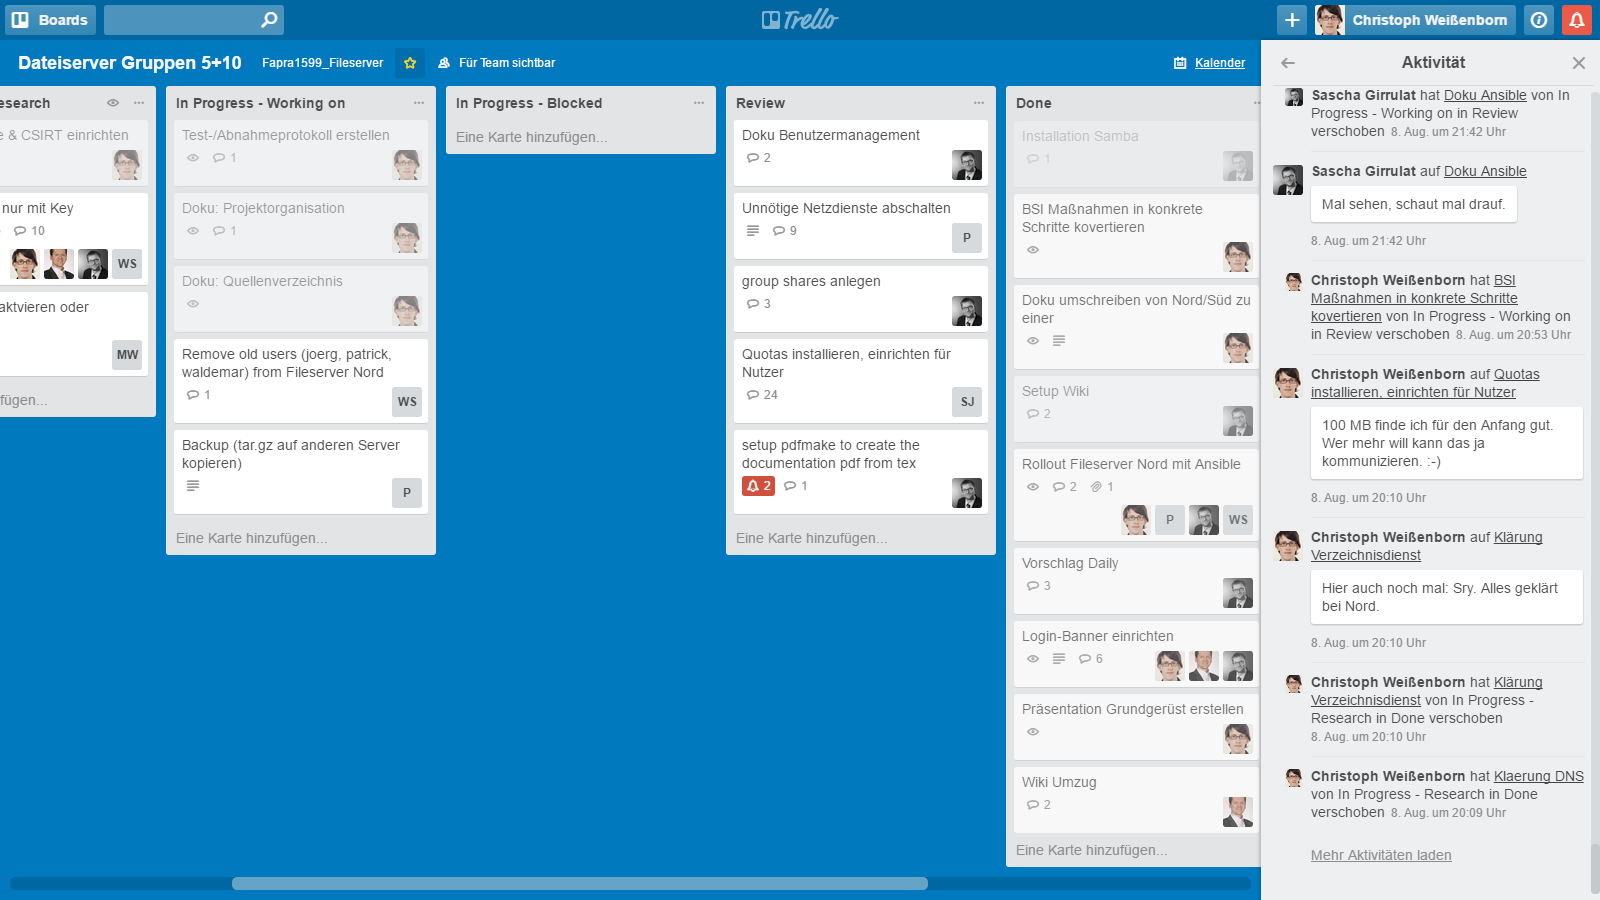
\includegraphics[scale=0.23]{images/trello.png}
	\caption[Screenshot des Kanban Board Trello für beide Gruppen]{Kanban Board Trello für beide Gruppen}
	\label{fig:nettop}
\end{figure}

Trello unterstützt nicht alle Praktiken, bietet aber ein kostenloses und einfaches Setup für alle Teilnehmer. Um fehlende Funktionen -- wie etwa die Begrenzung der angefangenen Arbeit -- abzudecken, haben wir an deren Stelle entsprechende organisatorische Regelungen getroffen.

\paragraph{Begrenze die Menge angefangener Arbeit:}Die Anzahl der Trello Tickets, die gleichzeitig bei einem PMA in Bearbeitung sind, darf bei uns nicht mehr als zwei betragen. Hierdurch entsteht ein Pull-System, bei dem sich jeder PMA seine Arbeit bei der Vorgängerstation abholt, anstatt fertige Arbeit einfach an die nächste Station zu übergeben.\footcite{wikiKanban}

\paragraph{Mache die Regeln für den Prozess explizit:}Um sicherzustellen, dass alle Beteiligten des Prozesses wissen, unter welchen Annahmen und Gesetzmäßigkeiten man arbeitet, werden möglichst alle Regeln, die es gibt, explizit gemacht. Dazu gehören z.B.
\begin{itemize}
\item eine Definition des Begriffes ‚fertig‘, ähnlich der Definition of Done in Scrum\footcite{wikiScrum},
\item Bedeutung der einzelnen Spalten,
\item Antworten auf die Fragen: wer zieht, wann zieht man, wie wählt man das nächste zu ziehende Ticket aus der Menge der vorhandenen Tickets aus, usw.\footcite{wikiKanban}
\end{itemize}

Enstsprechend der o.a. Punkte wurde eine gemeinsame \emph{Definition of Done} (siehe \ref{subsec:dod}) in Scrum sowie eine spezifizierte Abgrenzung der Trello-Spalten vorgenommen.

\begin{minipage}{\textwidth}
\captionof{table}{Von uns definierte Trello-Kategorien (Spalten)}
\begin{center}
\begin{tabular}{p{2.5cm}p{13cm}}
\toprule
Bezeichnung & Beschreibung \\
\midrule
Backlog & Aufgaben, die auf Bearbeitung warten. Hier kann jeder zugreifen und sich eine Aufgabe nehmen. Um zu verhindern, dass Arbeit doppelt gemacht wird, wird das Übernehmen der Aufgabe durch Hinzufügen der eigenen Person zur Aufgabe gekennzeichnet. Da die Zuordnung zu Personen erst in der nächsten Spalte passiert, ist die Taskanzahl hier noch nicht beschränkt. \\
In Progress - Research & Aufgaben, die in Bearbeitung sind und bei denen der Inhalt noch evaluiert werden muss, z.B. wenn noch nicht klar ist, wie etwas konkret umgesetzt werden muss. Hier sollte die Anzahl der Aufgaben pro Person zwei nicht überschreiten. \\
In Progress - Working on & Aufgaben, die konkret in Bearbeitung sind. Hier sollte die Anzahl der Aufgaben pro Person drei nicht überschreiten. \\
In Progress - Blocked & Die Aufgabe kann nicht weiter bearbeitet werden, etwa weil Zuarbeiten von anderen Personen fehlen oder technische Probleme eine weitere Bearbeitung verhindern. Die Anzahl der Aufgaben sollte pro Person fünf Aufgaben nicht überschreiten. \\
To Review & Um sicherzustellen, dass alle Aufgaben gemäß DoD mit einem 4-Augen Prinzip bearbeitet wurden, werden bearbeitete Tasks anschließend hierher verschoben. Jeder kann sich hier Aufgaben nehmen und sich den Inhalt entweder vorführen lassen oder selbständig anschauen und ggf. kommentieren oder ergänzen. Sollten Ergänzungen nötig sein, muss der Task entsprechend wieder in einen Zustand der Bearbeitung verschoben werden. Die Aufgabenanzahl sollte pro Person drei Aufgaben nicht überschreiten. \\
Done & Aufgabe ist gemäß DoD abgeschlossen. Taskanzahl ist unbegrenzt. \\
Ideas & Aufgaben mit niedrigster Priorität, die optional umzusetzen sind. Taskanzahl ist unbegrenzt. \\
\bottomrule
\end{tabular}
\end{center}
\end{minipage}

\paragraph{Miss und steuere den Fluss:} Die Mitglieder eines Kanban-Prozesses
messen typische Größen, wie Längen von Warteschlangen, Zykluszeit und Durchsatz,
um festzustellen, wie gut die Arbeit organisiert ist, wo man noch etwas
verbessern kann und welche Versprechen man an die Partner geben kann, für die
man arbeitet. Dadurch wird die Planung erleichtert und die Verlässlichkeit
gesteigert.\footcite{wikiKanban}

Im Rahmen unseres Projektes wurde der Projektfluss bei wöchentlichen
Mumble-Meetings besprochen und ggf. Maßnahmen zur Verbesserung eingeleitet.
Dabei war die enge Zusammenarbeit der Gruppen 5 und 10 von großer Bedeutung,
insbesondere da in Gruppe 10 nur 2 von 5 Kursteilnehmern auch tatsächlich für
das Projekt zur Verfügung standen. Weiterhin haben wir unterschiedliche
Prioritäten für die Kanban Tasks definiert (siehe
\ref{subsec:priorisierung}).\\

\paragraph{Fördere Leadership auf allen Ebenen in der Organisation:}
Verbesserung kann nur funktionieren, wenn sich alle Ebenen in der Organisation
daran beteiligen. Besonders wichtig ist es, dass Mitarbeiter, die direkt die
Arbeit verrichten, ``Acts of Leadership'' zeigen und konkrete
Verbesserungsvorschläge einbringen.\footcite{wikiKanban}\\

Damit der Prozess der kontinuierlichen Verbesserung in der Gruppe funktioniert,
ist die Mitwirkung aller Projektbeteiligten erforderlich. Verantwortung
sinnvoll übernehmen kann nur, wer auch die ihm übertragene Sache betreffende
Entscheidungen treffen und umsetzen darf.\\

In unserem Projekt sind alle PMA gleichberechtigte Partner. Jeder von uns ist
daher berechtigt alle Entscheidungen zu treffen, deren Verantwortung er sich
selbst zutraut. Einzige Bedingung ist, dass alle Entscheidungen und Maßnahmen
dokumentiert und den anderen PMA zur Überprüfung zur Verfügung gestellt werden.

\paragraph{Verwende Modelle, um Chancen für kollaborative Verbesserungen zu erkennen:}
Modelle sind Vereinfachungen über den Prozess. Ein beliebtes Modell ist z.B.
das von Wert, Fluss und Verschwendung aus der ``Lean IT''. Andere Modelle
basieren auf den Ideen von Deming oder auf der Engpasstheorie, auf systemischem
Denken oder auf der Komplexitätstheorie. Modelle können dabei helfen, ein
besseres Prozessverständnis zu erreichen und Experimente zu finden, die zu
einer Verbesserung des Prozesses führen.\footcite{wikiKanban}

Da der Fokus des Kurses auf der IT Sicherheit lag, haben wir uns entschlossen,
den von uns verwendeten Maßstab für die Sicherheit unserer Lösung (siehe
\ref{subsec:si}) auch als Maßstab für den Fortschritt des Projektes zu
verwenden.\footcite{wikiKanban} \\

Durch eine regelmäßige Überprüfung der dazu verwendeten Liste an Maßnahmen,
haben wir stockende oder noch offene Arbeitspakete identifiziert und bei den
regelmäßigen gemeinsamen Besprechungen den dafür notwendigen Arbeitsfluss
organisiert.

Die Visualisierung und die Begrenzung des Arbeitsflusses sind einfache Mittel,
mit denen rasch sichtbar wird, wie schnell die Tickets die verschiedenen
Stationen durchlaufen und wo sich Tickets stauen. Die Stellen, vor denen sich
Tickets häufen, während an den nachfolgenden Stationen freie Kapazitäten
vorhanden sind, werden als Bottlenecks bezeichnet. Durch Analysen des
Kanban-Boards können immer wieder Maßnahmen ergriffen werden, um einen
möglichst gleichmäßigen Fluss (Flow) zu erreichen. Beispielsweise können die
Limits für einzelne Stationen verändert werden, es können Puffer eingeführt
werden (insbesondere vor Bottlenecks, die durch nur zeitweise Verfügbarkeit von
Ressourcen entstehen), die Anzahl der Mitarbeiter an den verschiedenen
Stationen kann verändert werden, technische Probleme werden beseitigt usw.
Dieser kontinuierliche Verbesserungsprozess (japanisch: Kaizen) ist
wesentlicher Bestandteil von Kanban.\footcite{wikiKanban}\\

\subsection{Meetings}
\subsubsection{Status-Meetings}
Aufgrund der geografischen Verteilung und der unterschiedlichen Verfügbarkeit der Teammitglieder, werden wir die in der agilen Vorgehensweise üblichen, täglichen Statusmeetings in einer etwas geänderten Form abhalten. Alle Teilnehmer der Gruppen Dateiserver Nord und Süd treffen sich Mo,Mi,Fr um 20:00 für ein Statusmeeting von maximal 60 Minuten auf einem der vorhandenen Mumble Server. Hierbei gelten folgende Regeln:

\begin{itemize}
\item Das Meetings findet vor dem virtuellen Kanban Board statt
\item Jeder sollte seine Sprechzeit zum Status der eigenen Tasks auf 90 Sekunden beschränken
\item Jeder sollte innerhalb seiner Sprechzeit folgende Punkte durchgehen:
\begin{itemize}
\item Was habe ich seit dem letzten Treffen gemacht?
\item Was will ich bis zum nächsten Treffen machen?
\item Was blockiert mich bei meiner Arbeit?
\end{itemize}
\item Wenn einer spricht, hört die restliche Gruppe zu
\item Tasks sollten, wenn möglich, innerhalb des Meetings verschoben werden. Wenn die Aufgabenrestriktion der Spalten das nicht zulässt, können Tasks vorher schon auf Review gezogen werden, sollten aber nur innerhalb des Statusmeetings auf Done gezogen werden, damit alle einen gemeinsamen Wissensstand darüber haben, welche Aufgaben bereits abgeschlossen sind. Am Wochenende werden Statusmeetings nach Absprache gehalten.
\end{itemize}

\subsubsection{Review-Meetings}
Einmal in der Woche wird ein Review Meeting durchgeführt, bei dem alle PMA kurz für die Gruppen erläutern, was in der Zwischenzeit geschehen ist. Bei Bedarf können über Screen- oder Teamviewer-Sessions Dinge vorgeführt werden oder Probleme gemeinsam gelöst werden. Die Terminabsprache erfolgt immer innerhalb des Review Meetings für das darauf folgende. Wenn nötig, wird ein Protokoll geführt. Informationen hierzu werden im Wiki veröffentlicht. \\

Während des Review Meetings wird auch „Board Grooming“ durchgeführt. Dieser Vorgang ist aus Scrum als \textit{Backlog Grooming}\footcite{wikiScrum} bekannt, und beschreibt einen wiederkehrenden Prozess zur Überarbeitung und Weiterentwicklung des Backlogs. Wir werden hier ebenfalls einen für Kanban angepassten und vereinfachten Prozess anwenden, der folgende Punkte enthält:

\begin{itemize}
\item Ordnen und Zusammenfassen von Aufgaben auf dem Board
\item Löschen/Beenden von Einträgen, die nicht mehr wichtig sind
\item Hinzufügen von neuen Einträgen
\item Detaillieren von Aufgaben
\item ggf. nötige Planung von Rollouts
\item Zuordnen von Reviews
\item Beenden von abgeschlossenen Tasks
\end{itemize}

\subsection{Priorisierung}
\label{subsec:priorisierung}
Für die Entscheidung, welche Tasks zuerst durchgeführt werden müssen, werden in Kanban häufig die Verzögerungskosten (Cost of Delay) zu Rate gezogen\footcite{wikiKanban}. Da diese bei einem Projekt ohne Budget oder Gewinnabsicht jedoch sehr fiktiv sind, haben wir auf eine formelle Analyse hierzu verzichtet und die Priorisierung bei den wöchentlichen Meetings abgesprochen.

\subsubsection{Internes Service Level Agreement (Kanban SLA)}
In Kanban sind (optional) verschiedene Service-Arten (Classes of Service) vorgesehen, mit denen die Priorisierung der einzelnen Tasks geregelt werden kann. Wir haben diese, leicht verändert, auch bei uns realisiert.

\begin{minipage}{\textwidth}
\captionof{table}{Interne SLA Kategorien}
\begin{center}
\begin{tabular}{p{2.2cm}p{2.4cm}p{10.8cm}}
\toprule
Kanban \newline Bezeichnung & Unsere \newline Bezeichnung & Beschreibung \\
\midrule
Standard & Standard & Wird automatisch für alle nicht gekennzeichneten Tickets angenommen. \\
Expedite & Beschleunigt & Aufgaben, die mit dieser Priorität versehen werden, gefährden direkt den Erfolg des Projekts und haben Einfluss auf alle Beteiligten. Diese Aufgaben müssen unmittelbar von allen verfügbaren Mitgliedern bearbeitet werden. Direkt im Anschluss muss eine Information der anderen Mitglieder stattfinden und der Sachstand im Task vermerkt werden. Diese Priorität sollte nur in absoluten Ausnahmen vergeben werden. Diese Aufgaben werden mit einer roten Markierung versehen. \\
Intangible & Optional & Diese Aufgaben werden in der Spalte Ideen gesammelt und mit einer orangen Markierung versehen. Sie sind mit niedriger Priorität zu bearbeiten; solange noch Aufgaben mit höherer Priorität vorhanden sind, sollten diese nicht bearbeitet werden. Diese Aufgaben haben keinen Einfluss auf den Grad der Fertigstellung der eigentlichen Projektaufgabe.\\
Fixed Date & Fester \newline Termin & Wird in der Aufgabe mit einem Fälligkeitsdatum und einer blauen Markierung versehen. Die entsprechenden Tickets sollten so durch das Kanban-System geschleust werden, dass die Funktionalität kurz vor diesem Stichtag produktiv geht. \\
\bottomrule
\end{tabular}
\end{center}
\end{minipage}

\subsection{Gemeinsames Repository}
Um Code und technische Daten auszutauschen, nutzen wir ein öffentliches (Git-)Repository\footcite{githubRepo} auf Github. Um Änderungen durchführen zu können, bekommen alle Mitglieder der beiden Teams (auf Anforderung) entsprechende Berechtigungen.

\subsubsection{Motivation}
Unabhängig von dem expliziten Einsatz von Git, bietet uns ein Versionskontrollsystem folgende Vorteile\footcite{stackoverflowVersionControl}

\begin{itemize}
\item \textbf{Nachvollziehbarkeit}: Es kann jederzeit nachvollzogen werden, wer wann was geändert hat.
\item \textbf{Reversibilität}: Im Fehlerfall können Änderungen leichter herausgefunden und ggf. zurückgenommen werden.
\item \textbf{Synchronisation}: Gemeinsame Nutzung des Codes durch alle Teilnehmer.
\item \textbf{Kollaboration}: Gleichzeitige Arbeit an verschiedenen Features durch Branches.
\item \textbf{Vergleichbarkeit}: Durch die Archivierung aller Commits der Teilnehmer sind beispielsweise problemlos direkte Vergleiche zwischen verschiedenen Versionen möglich.
\end{itemize}

Wir haben uns für Github entschieden, da es
\begin{itemize}
\item kostenlosen Zugang für alle Teilnehmer ermöglicht
\item eine integrierte Benutzerverwaltung bietet
\item einfache Integration von externen Modulen (fork) vorsieht
\item durch Integrationstests via Travis-CI das Testen von Code erleichtert
\item ermöglicht, die technische Dokumentation durch eine bereits enthaltene Github-zu-Markdown-Schnittstelle einfach vorzubereiten
\item Zugriff auch ohne explizite Berechtigungen ermöglicht
\end{itemize}

\subsection{Konfigurationsmanagement-System}
Moderne Konfigurationsmanagement-Systeme arbeiten mit einer zentralen Komponente, in welcher der SOLL-Zustand der zu administrierenden Systeme (Zielsysteme) beschrieben wird. Dieses SOLL wird dann durch einen Zugriff auf die Zielsysteme mit dem IST-Zustand abgeglichen und kann auf diesem Wege auch direkt ausgerollt werden.

\subsubsection{Motivation}
Ein Konfigurationsmanagement-System bietet unserer Meinung nach - im Vergleich zur lokalen Administration der einzelnen Systeme - folgende Vorteile\footcite{whyCM}:

\begin{itemize}
\item \textbf{Skalierbarkeit}: Neue Server-Systeme können relativ einfach eingerichtet werden; die bestehende Konfiguration kann auf diese Systeme direkt ausgerollt werden
\item \textbf{Reproduzierbarkeit} und dadurch zeitnahe \textbf{Wiederherstellbarkeit}: Kommt es zu nicht nachvollziehbaren Fehlern auf einem Zielsystem, so kann dieses automatisiert wieder in einen definierten Zustand überführt werden. Selbst irreversible Fehler können durch eine komplette Neuinstallation der Systeme deutlich schneller behoben werden: Sobald das Betriebssystem installiert und per ssh erreichbar ist, kann die weitere Software-Installation und Konfiguration vollautomatisch vorgenommen werden. Auch der Austausch von Hardware ist so mit deutlich weniger Aufwand verbunden. In Verbindung mit organisatorischen Regelungen (siehe Betriebshandbuch) ist es uns möglich, mit dem (bei diesem Projekt zwangsläufig beschränkten) Personaleinsatz deutlich kürzere Wiederanlaufzeiten zu realisieren und eine höhere effektive Servicequalität zu gewährleisten.
\item \textbf{Verifikation} von Code vor der Implementierung: Ansible verfügt über eine „Check“-Option, welche es ermöglicht vor dem Rollout einer Konfiguration zu prüfen, an welchen Stellen genau dadurch eine Änderung auf den produktiven Systemen erfolgt.
\item \textbf{Systemunabhängigkeit}: Durch die deklarative Beschreibung der gewünschten Konfiguration ist das tatsächlich verwendete Zielsystem bei der Konfiguration transparent; so kann etwa SAMBA mit identischem Code auf zwei verschiedenen Linux-Distributionen ausgerollt werden.
\item Vereinigung von technischer \textbf{Dokumentation} und Konfiguration: Durch die deskriptive Art der Konfiguration, sowie durch die Möglichkeit Beschreibungen in der Konfiguration einzubauen, ist die Konfiguration auch für Personen nachvollziehbar, die nicht mit den technischen Besonderheiten der verwendeten Betriebssysteme und Softwarelösungen vertraut sind. Die Konfiguration dient so gleichzeitig der technischen Dokumentation. In Verbindung mit dem verwendeten Versionskontrollsystem (siehe 3.5) ist dadurch nachvollziehbar, wer wann welche Änderungen genau an den Produktivservern vorgenommen hat.
\item Darüber hinaus stellt es bei der Verwaltung von IT-Systemen einen erheblichen \textbf{Effizienzgewinn} dar, Konfiguration und Code zentral zur kollaborativen Bearbeitung zur Verfügung zu haben.
\end{itemize}

Es standen verschiedene Lösungen, wie z.B. Ansible\footcite{ansible}, Puppet\footcite{puppet} und Chef\footcite{chef} zur Diskussion. Unsere Gruppen haben sich aus folgenden Gründen\footcite{whyAnsible} für den Einsatz von Ansible entschieden:

\begin{itemize}
\item Vollumfänglicher Betrieb \textbf{ohne Management-Server oder speziellem Agent} auf den Zielsystemen möglich (anders als bei Puppet und Chef)
\item Einfache Syntax im yaml (\textbf{Markdown}) Format
(für Puppet und Chef sind umfangreichere Programmierkenntnisse erforderlich)
\item Geringe Anforderungen an das ausführende System - Es ist \textbf{lediglich python und ein ssh Client nötig} (Puppet und Chef benötigen z.B. viele Ruby Bibliotheken)
\item \textbf{kompatibel} mit allen verbreiteten Unix-Systemen (Linux, OpenBSD , Solaris,...)
\item „Push-Prinzip“ durch \textbf{Ausführung über SSH}; dadurch sind Releases leicht kontrollierbar und die Systeme einfach zugänglich und direkt integrierbar
(Puppet und Chef Arbeiten nach einem „Pull-Prinzip“)
\end{itemize}

Eine spätere Aufnahme von allen Systemen aus den Bereichen Nord und Süd ist nicht nur denkbar, sondern wird von uns auch ausdrücklich empfohlen. Das manuelle Installieren und Konfigurieren von Software in und auf produktiven Systemen ist ein in der Softwareentwicklung häufig anzutreffender, schlechter Lösungsansatz für ein bestimmtes Problem (Antipattern\footcite[S. 5-9]{humble2010continuous}).

\subsubsection{Verschlüsselung kritischer Codeblöcke}
\label{subsubsec:vault}
Ansible verfügt über die Möglichkeit schützenswerte Daten über PyCrypto zu verschlüsseln. Dieses Feature nennt sich \emph{Vault} und ermöglicht es alle Variablen in der Ansible üblichen Syntax in AES-verschlüsselten Dateien zu speichern. Diese werden dann zur Laufzeit der Konfiguration in den lokalen Kontext integriert. Hierzu muss ein „Vault-Password“ übergeben werden. \\

Alle schützenswerten Daten (z.b. die Zertifikate, initiale Benutzerpasswörter und Schlüssel) werden im Repository durch ein Vault verschlüsselt und mit einem entsprechend komplexen Passwort versehen. Dieses ist allen Teilnehmern bekannt. Bei Bedarf kann das Password PGP-verschlüsselt zur Verfügung gestellt werden und die verschlüsselten Dateien können mit einem neuen Passwort aktualisiert werden.

\begin{lstlisting}[label=code:labelname,caption=Auszug aus ansible/group\_vars/file\_server/public]
firstname: sascha
groups: sudo,file-sued,sshlogin,fapra1599,users
lastname: girrulat
name: sgirrulat
passwords:
  crypt: '{{ _vault_user_crypt_password["sgirrulat"] }}'
  plain: '{{ _vault_user_plain_password["sgirrulat"] }}'
\end{lstlisting}

\begin{lstlisting}[label=code:labelname,caption=Modifizierter Auszug aus ansible/group\_vars/file\_server/vault]
__vault_user_crypt_password:
  sgirrulat:        'xxxxxxx'

__vault_user_plain_password:
  sgirrulat:        'xxxxxxx'
\end{lstlisting}

Da sbmpasswd in Zusammenarbeit mit lokalen Benutzern nur mit Passwörtern in Klartext umgehen kann und Ansible nur mit Passwörtern im Crypt Format, mussten für alle Nutzerkonten die entsprechenden Passwörter in beiden Formaten erzeugt und gespeichert werden.

\newpage
\begin{minipage}{\textwidth}
\begin{center}
\captionof{table}{Übersicht der technischen Werkzeuge}
\begin{tabular}{lp{12cm}}
\toprule
Werkzeug & Verwendung für \\
\midrule
Trello &
  \begin{minipage}[t]{1\textwidth}
    \begin{itemize}
    \item Arbeitspaketierung
    \item Visualisierung des Arbeitsflusses (Kanban)
    \item Arbeitsflusssteuerung (Kanban)
    \item Verbesserungsvorschläge (Kanban: Leadership)
    \end{itemize}
  \end{minipage} \\
\midrule
DokuWiki &
  \begin{minipage}[t]{1\textwidth}
    \begin{itemize}
    \item Sammelstelle für Dokumentation
    \item Meeting-Protokolle
    \item Austausch komplexer Informationen mit anderen Gruppen
    \end{itemize}
  \end{minipage}\\
\midrule
Github Repository &
  \begin{minipage}[t]{1\textwidth}
    \begin{itemize}
    \item Zentrale Ablage aller Konfigurationen
    \item Konfliktbehebung bei paralleler Code-Bearbeitung
    \end{itemize}
  \end{minipage}\\
  \midrule
Travis CI &
  \begin{minipage}[t]{1\textwidth}
    \begin{itemize}
    \item Integrationstests
    \end{itemize}
  \end{minipage}\\
  \midrule
Mumble (VoIP) &
  \begin{minipage}[t]{1\textwidth}
    \begin{itemize}
    \item Telekonferenzsystem für Besprechungen
    \item Konfliktbehebung bei paralleler Code-Bearbeitung
    \end{itemize}
  \end{minipage}\\
  \midrule
Doodle &
  \begin{minipage}[t]{1\textwidth}
    \begin{itemize}
    \item Urlaubsplaner
    \end{itemize}
  \end{minipage}\\
  \midrule
Newsgroup k1599 &
  \begin{minipage}[t]{1\textwidth}
    \begin{itemize}
    \item multilateraler Austausch mit anderen Gruppen
    \item Anfragen an CIO
    \end{itemize}
  \end{minipage}\\
  \midrule
Dropbox &
  \begin{minipage}[t]{1\textwidth}
    \begin{itemize}
    \item gemeinsame Bearbeitung von Dokumentation \newline und Präsentation
    \item Backup aller Dokumente \newline(enthält nicht den technischen Code auf Github)
    \end{itemize}
  \end{minipage}\\
  \midrule
TeamViewer &
  \begin{minipage}[t]{1\textwidth}
    \begin{itemize}
    \item Videokonferenz für Besprechungen / Präsentationen
    \end{itemize}
  \end{minipage}\\
\bottomrule
\end{tabular}
\end{center}
\end{minipage}

\subsection{Zusammenarbeit mit anderen Gruppen}
Für die bilaterale Zusammenarbeit mit anderen Gruppen haben wir auf E-Mail gesetzt. Die multilaterale Mitwirkung haben wir über die Newsgroup angesteuert, da dies unserer Meinung nach der effizienteste Weg ist, alle Interessierten zu erreichen.

Für die Inbetriebnahme unseres Servers benötigten wir zunächst Informationen der Netzgruppen zu:
\begin{itemize}
\item IPv4 Konfiguration unserer Server
\item IPv6 Konfiguration unserer Server
\item DNS Anbindung
\item Active Directory
\end{itemize}
Diese Informationen haben wir zeitnah erhalten. Die für die CA zuständigen Gruppen haben uns die von ihnen benötigten Informationen jeweils proaktiv übermittelt, so dass wir unsere Server Mitte Juli im VPN in Betrieb nehmen konnten.\\

Es ist sinnvoll, einheitliche Betriebs- und Sicherheitsstandards in einer gesamten Produktivumgebung zu verwenden. Zu diesem Zweck haben wir den anderen Gruppen die Mitarbeit an einem gemeinsamen Betriebskonzept vorgeschlagen (30.07.16). Dieser Vorschlag blieb leider unbeantwortet, so dass wir die weiteren Arbeiten nur zwischen den Gruppen 5 und 10 abgesprochen haben.

\subsubsection{Information der Anwender}
Alle Kursteilnehmer haben eine E-Mail bekommen, mit der zum einen die Daten des
persönlichen Accounts mitgeteilt wurden und zum anderen der zugehörige
Gruppenbenutzer, z.B. ''cert-nord''. Für alle Benutzer wurde ein individuelles
Password erzeugt und zugeordnet. Ebenfalls gibt es für jede Gruppe einen
eigenen Benutzer, bei dem das Password nur den entsprechenden
Gruppen-Mitgliedern bekannt gemacht wurde.\\

\textbf{Vorlage:}
\begin{center}
\begin{framedminipage}{0.8\textwidth}
Sehr geehrte(r) KursteilnehmerIn,\\

auf den Servern der FileNord und FileSued wurden zwei Benutzer fuer Sie
angelegt. Hierbei handelt es sich zum Einen, um einen personalisierten Benutzer
fuer Sie und zum Anderen, um einen Benutzer fuer ihre Gruppe.\\
Persoenlicher Benutzer:\bigskip

  name: \{\{ user\_name \}\}
  password: \{\{ user\_password \}\}\bigskip

Gruppen Benutzer:\bigskip

  name: \{\{ group\_name \}\}
  password: \{\{ group\_password \}\}\bigskip

Bitte gehen Sie mit diesen Daten sorgsam um, da insbesondere das Passwort des
persoenlichen Benutzers nur Ihnen mitgeteilt wird.\\

Weitere Informationen folgen in separaten Benachrichtigungen.\\

Viel Erfolg\\

Gruppe FileNord und Gruppe FileSued
\end{framedminipage}
\end{center}

%----------------------------------------------------------------------------------------
%	SECTION FUNKTIONALES KONZEPT
%----------------------------------------------------------------------------------------
\newpage
\section{Funktionales Grobkonzept}

\subsection{Hardware}
\label{subsec:hardware}
Aufgrund des nicht vorhandenen Projektbudgets haben wir uns entschieden, zwei Server zu verwenden, welche schon im Vorfeld von unseren Mitgliedern angemietet wurden:

\begin{minipage}{\textwidth}
\begin{center}
\captionof{table}{Verwendete Server}
\begin{tabular}{llll}
\toprule
Service & Bereitgestellt von & Hosting Provider & Betriebssystem \\
\midrule
Datei Nord & Jörg Ricardo Schumacher & netcup GmbH & Ubuntu 16.04 LTS \\
Datei Süd & Sascha Girrulat & Hetzner Online GmbH & Debian GNU/Linux 8.5 \\
\bottomrule
\end{tabular}
\end{center}
\end{minipage}\bigskip

Wo sich diese -- aus finanziellen Erwägungen getroffene -- Entscheidung später auf das Sicherheitskonzept auswirkt, haben wir dies entsprechend dokumentiert.

\subsection{Dateiservice}
Zur Überlegung standen mehrere Softwarelösungen zur Bereitstellung von Dateidiensten:

\begin{itemize}
\item SAMBA (SMB)
\item OwnCloud (HTTP/HTTPS/WebDAV/FTP)
\item SeaFile (HTTP/HTTPS)
\item ProFTPD (FTP)
\end{itemize}
Wir haben uns schließlich entschlossen SAMBA\footcite{samba} zu nutzen und den Dateizugriff via SMB/CIFS zu ermöglichen. Für diese Lösung haben wir uns entschlossen, da SAMBA:

\begin{itemize}
\item eine erprobte und weit entwickelte Softwarelösung ist
\item die Anbindung an ein Active Directory nativ unterstützt
\item über die Kommandozeile aus der Ferne administriert werden kann
\item Transportverschlüsselung unterstützt (AES-CCM-128)
\item für fast alle Unix-Derivate (auf dem Server) verfügbar ist
\item SMB/CIFS-Freigaben bietet, die sowohl unter Windows, als auch Linux direkt in die Verzeichnisstruktur des Clients eingebunden werden können, so dass aus jeder Anwendung heraus direkt das Speichern und Laden vom Server möglich ist
\item auch langfristig keine Lizenzkosten verursacht
\end{itemize}

%----------------------------------------------------------------------------------------
%	SECTION SICHERHEITSKONZEPT
%----------------------------------------------------------------------------------------
\newpage
\section{Sicherheitskonzept}
\label{sec:sicherheitskonzept}
Es existiert eine Vielzahl von IT-Sicherheitsstandards\footcite{wikiCyberSecStandards}. Das vorliegende Sicherheitskonzept richtet sich nach den Leitlinien des \emph{BSI IT-Grundschutz}\footcite{grundschutz}.\\

Kernziel des Projektes ist die Inbetriebnahme zweier Dateiserver. Daher werden im Folgenden nur Grundschutzaspekte modelliert, die für den sicheren Betrieb des Dateiservices -- mittelbar oder unmittelbar -- relevant sind. Die Absicherung anderer Teilaspekte der Gesamtumgebung -- wie auch die Absicherung der Gesamtumgebung an sich -- bleibt dabei unberücksichtigt. Eine abschließende Zertifizierung nach ISO/IEC 27001 ist nicht Bestandteil des Projektumfangs.\\

Aus technischer Sicht basiert das Sicherheitskonzept auf der \emph{Philosophie der Verteidigung in der Tiefe (Defense in depth)}\footcite{wikiDiD}\footcite{kuipers2006control}: Wir verlassen uns nicht auf eine einzelne Sicherheitsmaßnahme (Aus eigener Anschauung kennen wir die Argumentation "`Wir brauchen kein gutes Passwort, der Server steht doch hinter der Firewall"' von Administratoren mit sicherheitskritischen Aufgaben), sondern versuchen einem potentiellen Angreifer stets mehrere (voneinander unabhängige) Hürden in den Weg zu stellen. Da aus Ressourcengründen nur jeweils ein Server für Nord und einer für Süd verwendet wird, sind die Möglichkeiten der praktischen Umsetzung hierzu natürlich auf Softwarelösungen beschränkt.

\subsection{Security Index}
\label{subsec:si}
Dem Thema Sicherheit kommt in diesem Projekt eine besondere Bedeutung zu und die Absicherung der Systeme nimmt deutlich mehr Zeit in Anspruch, als die Bereitstellung der Funktionalität für den Anwender. Wir haben uns daher entschlossen, den Fortschritt des Projektverlaufes daran zu messen, inwieweit wir den Schutzbedarf der Anwendungen erfüllt haben. Um dies an einem einfachen, leicht zu visualisierenden Maßstab messen zu können, haben wir eine eigene Metrik entwickelt: Den Security Index (SI). Dieser ist wie folgt definiert:\\

Seien
\begin{itemize}
\item $n$ die Anzahl der von uns identifizierten BSI IT-Grundschutz Maßnahmen
\item $m_i$ die i-te Grundschutz-Maßnahme aus der Tabelle \ref{tab:massnahmen} im Anhang
\item $siv(m_i)$ (Security Index Value) das Gewicht \footnote{Motivation der Gewichtung: Die tatsächliche Effektivität und Wirksamkeit von technischen Maßnahmen ist leichter zu überprüfen, als die von rein organisatorischen Festlegungen („Papier ist geduldig“)} der $i$-ten Maßnahme mit
\begin{equation}
siv(x)=
\begin{cases}
    0,& \text{wenn Dateiserverguppen nicht verantwortlich für $x$ }\\
    1,& \text{wenn $x$ organisatorische Maßnahme}\\
    2,& \text{wenn $x$ technische Maßnahme von normaler Bedeutung}\\
    4,& \text{wenn $x$ technische Maßnahme von herausragender Bedeutung}
\end{cases}
\end{equation}
\item $f(m_i)$ der Grad der Erfüllung der Maßnahme (zwischen $0$ und $1$), zu entnehmen aus der folgenden Tabelle: \\

\begin{minipage}{\textwidth}
\begin{center}
\captionof{table}{Maßnahmenstatus}
\begin{tabular}{ll}
\toprule
Maßnahmenstatus & SI Faktor \\
\midrule
abgeschlossen & 1,0 \\
abgeschlossen mit Restrisiken & 0,8 \\
Betriebshandbuch & 1,0 \\
externer Dienstl. & 1,0 \\
Hardening verboten & 1,0 \\
nicht zutreffend & 1,0 \\
nur organisatorisch & 0,5 \\
geplant & 0,0 \\
nicht durchgeführt & 0,0 \\
offen & 0,0 \\
Rollout & 0,0  \\
\bottomrule
\end{tabular}
\end{center}
\end{minipage}
\end{itemize}
\bigskip

dann ist der Sicherheitsindex

\begin{center}
\begin{equation}
SI:=\frac{\sum_{i=1}^n siv(m_i)\times f(m_i)}{\sum_{i=1}^{n}siv(m_i)}
\end{equation}
\end{center}

Ein SI von $1,0$ bedeutet also, dass alle vom BSI IT Grundschutz vorgeschlagenen Maßnahmen umgesetzt wurden (soweit sie für den Dateiserver-Betrieb relevant sind). Die aktuelle Entwicklung des SI haben wir in unregelmäßigen Abständen -- mindestens jedoch einmal wöchentlich -- dokumentiert. Der zum Abgabetermin wirksame SI ist $0,95$.\\

Der SI kann und soll eine eingehende Betrachtung der aktuellen Sicherheitslage nicht ersetzen. Für eine grobe Abschätzung der IT Sicherheitsvorkehrungen, wie sie etwa im Management erforderlich ist, kann dieser Index jedoch genutzt werden.

\begin{figure}[hbt!]
		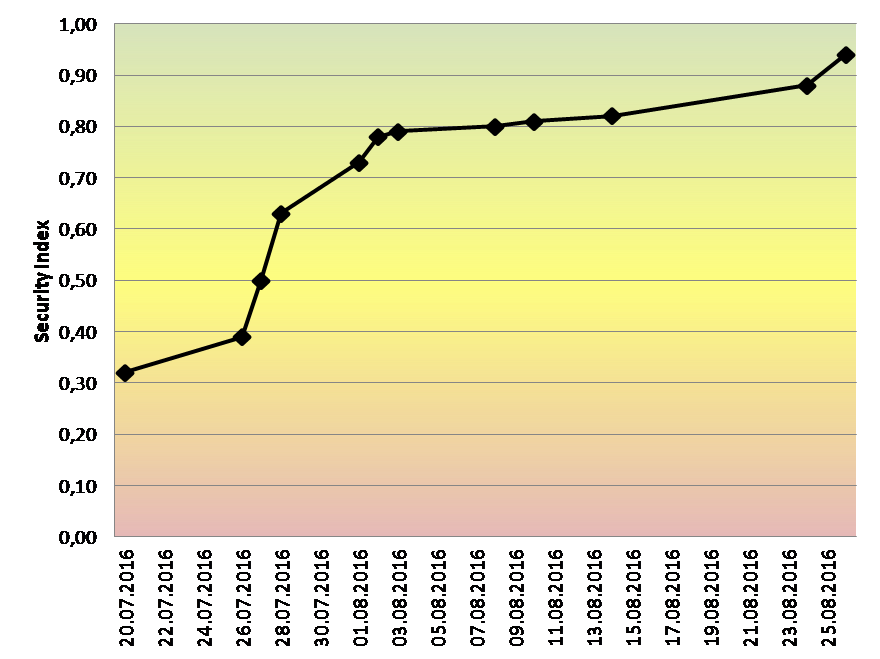
\includegraphics[scale=0.66]{images/si.png}
	\caption{Security Index (SI) im Projektverlauf}
	\label{img:si}
\end{figure}

\subsection{Schutzbedarfsfeststellung}
\label{subsec:schutzbedarfsfeststellung}
\begin{minipage}{\textwidth}
\begin{center}
\captionof{table}{Definition von Schutzbedarfskategorien}
\begin{tabular}{lp{14cm}}
\toprule
Kategorie & Definition \\
\midrule
Normal & Die Schadensauswirkungen sind begrenzt (etwa auf eine einzelne Verkaufsstelle) und überschaubar. \newline Die maximal tragbare Ausfallzeit übersteigt vier Tage.\\[0.3cm]
Hoch & Die Schadensauswirkungen können beträchtlich sein und z.B. zum Ausfall eines einzelnen Dienstes für alle Verkaufsstellen führen. \newline Die maximal tragbare Ausfallzeit beträgt zwischen zwei und vier Tagen. \\[0.3cm]
Sehr hoch & Die Schadensauswirkungen können den Bestand der vereinigten Back-werke existentiell bedrohen oder das Betriebsergebnis des Jahres katastrophal beschädigen. \newline Die maximal tragbare Ausfallzeit liegt unter zwei Tagen. \\
\bottomrule
\end{tabular}
\end{center}
\end{minipage}
\bigskip

\begin{minipage}{\textwidth}
\begin{center}
\captionof{table}{Schutzziele und Grundwerte}
\begin{tabular}{lp{14cm}}
\toprule
Grundwert & Definition der Verletzung \\
\midrule
Vertraulichkeit & Vertrauliche Informationen werden unberechtigt zur Kenntnis genommen oder weitergegeben. \\
Integrität & Die Korrektheit der Informationen und der Funktionsweise von Systemen ist nicht mehr gegeben. \\
Verfügbarkeit & Autorisierte Benutzer werden am Zugriff auf Informationen und Systeme behindert. \\
\bottomrule
\end{tabular}
\end{center}
\end{minipage}

\subsubsection{Schutzbedarf: Anwendungen}
\begin{minipage}{\textwidth}
\begin{center}
\captionof{table}{Anwendung Dateiserver}
\begin{tabular}{p{3.5cm}llp{6.3cm}}
\toprule
Anwendung & Grundwert & Schutzbedarf & Begründung \\
\midrule
Personaldaten-verwaltung & Vertraulichkeit & Hoch & Personaldaten sind besonders schutzbedürftige personenbezogene Daten, deren Bekanntwerden die Betroffenen erheblich beeinträchtigen könnte. \\
Personaldaten-verwaltung & Integrität & Normal & da Fehler rasch erkannt und die Daten nachträglich korrigiert werden können. \\
Personaldaten-verwaltung & Verfügbarkeit & Gering & Ausfälle von bis zu einer Woche können mittels manueller Verfahren überbrückt werden. \\
Finanzverwaltung & Vertraulichkeit & Hoch & Mit den Finanzdaten ist ein Zugriff auf die Konten der vereinigten Backwerke möglich. \\
Finanzverwaltung & Integrität & Hoch & Falsche oder fehlende Abrechnungen führen zu unbezahlten oder unbearbeiteten Bestellungen. \\
Finanzverwaltung & Verfügbarkeit & Normal & Rechnungen müssen nur innerhalb der üblichen Laufzeiten bezahlt werden. \\
Kassensystem & Vertraulichkeit & Gering & Backwerk-Bestellungen sind für unsere Kunden keine vertraulichen Informationen. \\
Kassensystem & Integrität & Normal & Falsche oder fehlende Kassendaten machen die Nachvollziehbarkeit von Ausgaben und Einnahmen unmöglich. \\
Kassensystem & Verfügbarkeit & Normal & Die Synchronisation der Kassenbestände erfolgt nachts und ist für den Tagesbetrieb nicht relevant.\\
\bottomrule
\end{tabular}
\end{center}
\end{minipage}

\subsubsection{Schutzbedarf: IT-Systeme}
\begin{minipage}{\textwidth}
\begin{center}
\captionof{table}{Anwendung Dateiserver}
\begin{tabular}{lll}
\toprule
Grundwert & Schutzbedarf & Begründung \\
\midrule
Vertraulichkeit & Hoch & Maximumprinzip \\
Integrität & Hoch & Maximumprinzip \\
Verfügbarkeit & Normal & Maximumprinzip \\
\bottomrule
\end{tabular}
\end{center}
\end{minipage}

\subsubsection{Schutzbedarf: Kommunikationsverbindungen}
\begin{minipage}{\textwidth}
\begin{center}
\captionof{table}{Anwendung Dateiserver}
\begin{tabular}{p{3cm}llp{6.8cm}}
\toprule
Anwendung & Grundwert & Schutzbedarf & Begründung \\
Dateiserver zu LAN-Client & Vertraulichkeit & Hoch & Maximumprinzip \\
 & Integrität & Hoch & Maximumprinzip \\
 & Verfügbarkeit & Normal & Maximumprinzip \\
Dateiserver zu Internet & Vertraulichkeit & Hoch & Kommunikation findet hier ausschließlich zur LAN-Anbindung statt \\
 & Integrität & Hoch &  \\
 & Verfügbarkeit & Normal &  \\
Dateiserver zu AD/DNS-Server & Vertraulichkeit & Hoch & Nutzer-Login-Daten \\
 & Integrität & Hoch & Nutzer-Authentifizierung \\
 & Verfügbarkeit & Normal &  \\
\bottomrule
\end{tabular}
\end{center}
\end{minipage}
\bigskip

\subsubsection{Schutzbedarf: Räume}
Entfällt, da hierfür - aus Kostengründen - auf einen bereits festgelegten externen Dienstleister gesetzt wird, bei dem die Konditionen nicht verhandelbar sind (siehe \ref{subsec:hardware}).

\subsection{Bausteine}
\begin{minipage}{\textwidth}
\begin{center}
\captionof{table}{Modellierung übergeordneter Aspekte}
\begin{tabular}{p{1cm}p{5cm}p{9cm}}
\toprule
Kürzel 	& Titel & Bemerkungen \\
\midrule
B1.3 	& Notfallvorsorgekonzept & \\
B1.4 	& Datensicherungskonzept & \\
B1.6 	& Computer-Viren-Schutzkonzept & \\
B1.7 	& Kryptokonzept	& \\
B1.8 	& Behandlung von \newline Sicherheitsvorfällen & Geregelt im Betriebshandbuch \\
\bottomrule
\end{tabular}
\end{center}
\end{minipage}
\bigskip

\begin{minipage}{\textwidth}
\begin{center}
\captionof{table}{Modellierung der Infrastruktur}
\begin{tabular}{p{1cm}p{5cm}p{9cm}}
\toprule
Kürzel 	& Titel & Bemerkungen \\
\midrule
B2.1 	& Gebäude & Server stehen in Rechenzentrum der netcup GmbH (Nord), bzw. Hetzner Online GmbH (Süd); im Weiteren daher nicht mit betrachtet \\
B2.2 	& Elektrotechnische \newline Verkabelung & Server stehen in Rechenzentrum der netcup GmbH (Nord), bzw. Hetzner Online GmbH (Süd); im Weiteren daher nicht mit betrachtet \\
B2.4 	& Serverraum & Server stehen in Rechenzentrum der netcup GmbH (Nord), bzw. Hetzner Online GmbH (Süd); im Weiteren daher nicht mit betrachtet \\
B2.5 	& Datenträgerarchiv	& Server stehen in Rechenzentrum der netcup GmbH (Nord), bzw. Hetzner Online GmbH (Süd); im Weiteren daher nicht mit betrachtet \\
B2.7 	& Schutzschränke & Geregelt im Betriebshandbuch Server stehen in Rechenzentrum der netcup GmbH (Nord), bzw. Hetzner Online GmbH (Süd); im Weiteren daher nicht mit betrachtet \\
\bottomrule
\end{tabular}
\end{center}
\end{minipage}
\bigskip

\begin{minipage}{\textwidth}
\begin{center}
\captionof{table}{Modellierung der IT-Systeme}
\begin{tabular}{p{1cm}p{5cm}p{9cm}}
\toprule
Kürzel 	& Titel & Bemerkungen \\
\midrule
B1.3 	& Notfallvorsorgekonzept & \\
B1.4 	& Datensicherungskonzept & \\
B1.6 	& Computer-Viren-Schutzkonzept & \\
B1.7 	& Kryptokonzept	& \\
B1.8 	& Behandlung von \newline Sicherheitsvorfällen & Geregelt im Betriebshandbuch \\
\bottomrule
\end{tabular}
\end{center}
\end{minipage}
\bigskip

\begin{minipage}{\textwidth}
\begin{center}
\captionof{table}{Modellierung der Anwendungen}
\begin{tabular}{p{1cm}p{5cm}p{9cm}}
\toprule
Kürzel 	& Titel & Bemerkungen \\
\midrule
B5.8	& Telearbeit	& Relevant für die sichere Einbindung der Clients \\
B5.17	& Samba			& \\
B5.18	& DNS-Server	& Betrieben durch Netzgruppen; im weiteren daher unberücksichtigt \\
B5.19	& Internet-Nutzung	& \\
B5.22	& Protokollierung	& \\
B5.23	& Cloud Management	& Basiert auf IETF Cloud Reference Framework \\
B5.25	& Allgemeine Anwendungen	& \\
B5.26	& Serviceorientierte Architektur	& \\
\bottomrule
\end{tabular}
\end{center}
\end{minipage}

\subsection{Maßnahmen}
Die Maßnahmen, welche sich aus den modellierten Bausteinen ergeben, sind in der Tabelle \ref{tab:massnahmen} „Identifizierte Maßnahmen“ zusammengefasst; dort ist auch der aktuelle Status der Maßnahme dokumentiert. Nähere Informationen (genaue Definition, Fachbegriffe, Beispiele technischer Konfiguration) lassen sich im IT-Grundschutz Handbuch\footcite{grundschutz} finden.\\

Alle letztendlich durchgeführten technischen Maßnahmen sind in der technischen Systembeschreibung (siehe \ref{sec:techsys}) aufgeführt. Alle organisatorischen Maßnahmen auf der administrativen Seite sind in den Betriebs- und Serviceprozessen des Betriebshandbuches (im Anhang) dokumentiert;  die vom Anwender zu beachtenden Regelungen sind analog in der „IT Richtlinie für Anwender“ (ebenfalls im Anhang) aufgelistet. Die restlichen Maßnahmen - d.h. jene, die wir analysiert haben, aber im Rahmen des Projektes nicht durchführen konnten - sind im Ausblick (Kapitel \ref{sec:ausblick}) aufgelistet.

\captionof{table}{Identifizierte Maßnahmen}
\label{tab:massnahmen}
\begin{longtable}{lp{3.7cm}|p{3cm}l|p{3.8cm}}
\toprule
Kürzel & Titel & Status & Verantwortung & Bemerkungen \\
\midrule
M1.28 & Lokale unterbrechungsfreie Stromversorgung & externer Dienstl. & 5+10 & Server gemietet bei netcup GmbH (Nord), bzw. Hetzner Online GmbH (Süd) \\
M2.137 & Beschaffung eines geeigneten Datensicherungssystems & nicht durchgeführt & 5+10 & aus Zeit- und Kostengründen nur teilweise realisiert \\
M2.138 & Strukturierte Datenhaltung & abgeschlossen & 5+10 &  \\
M2.154 & Erstellung eines Sicherheitskonzeptes gegen Schadprogramme & abgeschlossen & 5+10 &  \\
M2.157 & Auswahl eines geeigneten Viren-Schutzprogramms & abgeschlossen & 5+10 &  \\
M2.158 & Meldung von Schadprogramm-Infektionen & Betriebshandbuch & 5+10 &  \\
M2.159 & Aktualisierung der eingesetzten Viren-Schutzprogramme und Signaturen & abgeschlossen & 5+10 &  \\
M2.160 & Regelungen zum Schutz vor Schadprogrammen & abgeschlossen & 5+10 &  \\
M2.205 & Übertragung und Abruf personenbezogener Daten & abgeschlossen & 5+10 &  \\
M2.22 & Hinterlegen des Passwortes & abgeschlossen & 5+10 &  \\
M2.224 & Vorbeugung gegen Schadprogramme & abgeschlossen & 5+10 &  \\
M2.273 & Zeitnahes Einspielen sicherheitsrelevanter Patches und Updates & Hardening verboten & 5+10 &  \\
M2.31 & Dokumentation der zugelassenen Benutzer und Rechteprofile & abgeschlossen & 5+10 & via Ansible \\
M2.314 & Verwendung von hochverfügbaren Architekturen für Server & externer Dienstl. & 5+10 & Server gemietet bei netcup GmbH (Nord), bzw. Hetzner Online GmbH (Süd) \\
M2.315 & Planung des Servereinsatzes & abgeschlossen & 5+10 &  \\
M2.316 & Festlegen einer Sicherheitsrichtlinie für einen allgemeinen Server & Betriebshandbuch & 5+10 &  \\
M2.317 & Beschaffungskriterien für einen Server & externer Dienstl. & 5+10 & Server gemietet bei netcup GmbH (Nord), bzw. Hetzner Online GmbH (Süd) \\
M2.318 & Sichere Installation eines IT-Systems & abgeschlossen & 5+10 &  \\
M2.32 & Einrichtung einer eingeschränkten Benutzerumgebung & abgeschlossen & 5+10 &  \\
M2.33 & Aufteilung der Administrationstätigkeiten unter Unix & nicht durchgeführt & 5+10 & alle in der Gruppe haben volle Admin-Rechte \\
M2.34 & Dokumentation der Veränderungen an einem bestehenden System & Betriebshandbuch & 5+10 &  \\
M2.35 & Informations-beschaffung über Sicherheitslücken des Systems & Betriebshandbuch & 5+10 &  \\
M2.351 & Planung von Speicherlösungen & abgeschlossen mit Restrisiken & 5+10 & keine zentralen Mgmt Systeme \\
M2.354 & Einsatz einer hochverfügbaren SAN-Lösung & nicht zutreffend & 5+10 & Verfügbarkeitsanforderung nicht Sehr hoch \\
M2.358 & Dokumentation der Systemeinstellungen von Speichersystemen & abgeschlossen & 5+10 &  \\
M2.359 & Überwachung und Verwaltung von Speicherlösungen & geplant & 5+10 &  \\
M2.360 & Sicherheits-Audits und Berichtswesen bei Speichersystemen & Betriebshandbuch & 5+10 &  \\
M2.362 & Auswahl einer geeigneten Speicherlösung & abgeschlossen & 5+10 &  \\
M2.437 & Planung des Einsatzes eines Samba-Servers & abgeschlossen & 5+10 &  \\
M2.438 & Sicherer Einsatz externer Programme auf einem Samba-Server & abgeschlossen & 5+10 &  \\
M2.46 & Geeignetes Schlüsselmanagement & nur Organisatorisch & 5+10 & Server voll, Client nur Org. \\
M2.525 & Erstellung einer Sicherheitsrichtlinie für Speicherlösungen & abgeschlossen & 5+10 &  \\
M2.526 & Planung des Betriebs der Speicherlösung & Betriebshandbuch & 5+10 &  \\
M2.527 & Sicheres Löschen in SAN-Umgebungen & externer Dienstl. & 5+10 & Server gemietet bei netcup GmbH (Nord), bzw. Hetzner Online GmbH (Süd) \\
M2.528 & Planung der sicheren Trennung von Mandanten in Speicherlösungen & nicht zutreffend & 5+10 & Es existiert nur je ein Mandant \\
M2.529 & Modellierung von Speicherlösungen & abgeschlossen & 5+10 &  \\
M3.23 & Einführung in kryptographische Grundbegriffe & abgeschlossen & 5+10 & alle Anwender sind Admins \\
M3.54 & Schulung der Administratoren des Speichersystems & abgeschlossen & 5+10 &  \\
M3.68 & Schulung der Administratoren eines Samba-Servers & abgeschlossen & 5+10 &  \\
M3.69 & Einführung in die Bedrohung durch Schadprogramme & abgeschlossen & 5+10 &  \\
M3.92 & Grundlegende Begriffe beim Einsatz von Speicherlösungen & abgeschlossen & 5+10 &  \\
M4.105 & Erste Maßnahmen nach einer Unix-Standardinstallation & Hardening verboten & 5+10 &  \\
M4.106 & Aktivieren der Systemprotokollierung & abgeschlossen & 5+10 & rsyslog \\
M4.13 & Sorgfältige Vergabe von IDs & abgeschlossen & 5+10 &  \\
M4.14 & Obligatorischer Passwortschutz unter Unix & abgeschlossen & 5+10 &  \\
M4.15 & Gesichertes Login & abgeschlossen mit Restrisiken & 5+10 & ausgenommen Meldung des letzten erfolglosen Login \\
M4.16 & Zugangs-beschränkungen für Benutzer-Kennungen und / oder Terminals & nicht zutreffend & 5+10 & keine festen Arbeitszeitfenster \\
M4.17 & Sperren und Löschen nicht benötigter Accounts und Terminals & Betriebshandbuch & 5+10 &  \\
M4.18 & Administrative und technische Absicherung des Zugangs zum Monitor- und Single-User-Modus & externer Dienstl. & 5+10 &  \\
M4.19 & Restriktive Attributvergabe bei Unix-Systemdateien und -verzeichnissen & abgeschlossen & 5+10 &  \\
M4.20 & Restriktive Attributvergabe bei Unix-Benutzerdateien und -verzeichnissen & abgeschlossen & 5+10 &  \\
M4.21 & Verhinderung des unautorisierten Erlangens von Administratorrechten & abgeschlossen & 5+10 &  \\
M4.22 & Verhinderung des Vertraulichkeitsverlusts schutzbedürftiger Daten im Unix-System & abgeschlossen & 5+10 & Login am System beschränkt auf Admins \\
M4.23 & Sicherer Aufruf ausführbarer Dateien & abgeschlossen mit Restrisiken & 5+10 & PATH nicht überwacht \\
M4.237 & Sichere Grundkonfiguration eines IT-Systems & abgeschlossen & 5+10 & Integritätsdatenbank = Ansible \\
M4.238 & Einsatz eines lokalen Paketfilters & abgeschlossen & 5+10 &  \\
M4.239 & Sicherer Betrieb eines Servers & Betriebshandbuch & 5+10 &  \\
M4.24 & Sicherstellung einer konsistenten Systemverwaltung & abgeschlossen & 5+10 &  \\
M4.240 & Einrichten einer Testumgebung für einen Server & nicht zutreffend & 5+10 & Verfügbarkeitsanforderung nicht Sehr hoch \\
M4.25 & Einsatz der Protokollierung im Unix-System & abgeschlossen & 5+10 &  \\
M4.26 & Regelmäßiger Sicherheitscheck des Unix-Systems & nur Organisatorisch & 5+10 & keine automatisierte Prüfung \\
M4.274 & Sichere Grundkonfiguration von Speichersystemen & abgeschlossen & 5+10 &  \\
M4.275 & Sicherer Betrieb einer Speicherlösung & Betriebshandbuch & 5+10 &  \\
M4.3 & Einsatz von Viren-Schutzprogrammen & abgeschlossen & 5+10 &  \\
M4.305 & Einsatz von Speicherbeschränkungen (Quotas) & Betriebshandbuch & 5+10 &  \\
M4.326 & Sicherstellung der NTFS-Eigenschaften auf einem Samba-Dateiserver & abgeschlossen & 5+10 &  \\
M4.327 & Überprüfung der Integrität und Authentizität der Samba-Pakete und -Quellen & abgeschlossen & 5+10 &  \\
M4.328 & Sichere Grundkonfiguration eines Samba-Servers & abgeschlossen & 5+10 &  \\
M4.329 & Sicherer Einsatz von Kommunikationsprotokollen beim Einsatz eines Samba-Servers & abgeschlossen & 5+10 &  \\
M4.330 & Sichere Installation eines Samba-Servers & abgeschlossen & 5+10 &  \\
M4.331 & Sichere Konfiguration des Betriebssystems für einen Samba-Server & abgeschlossen & 5+10 &  \\
M4.332 & Sichere Konfiguration der Zugriffssteuerung bei einem Samba-Server & abgeschlossen & 5+10 &  \\
M4.333 & Sichere Konfiguration von Winbind unter Samba & nicht zutreffend & 5+10 & kein AD eingerichtet \\
M4.334 & SMB Message Signing und Samba & abgeschlossen & 5+10 & da nur als Dateiserver genutzt kann Default bleiben \\
M4.335 & Sicherer Betrieb eines Samba-Servers & abgeschlossen & 5+10 &  \\
M4.432 & Sichere Konfiguration von Serverdiensten & abgeschlossen & 5+10 & Authentisierung intern unverschlüsselt \\
M4.433 & Einsatz von Datenträgerverschlüsselung & externer Dienstl. & 5+10 &  \\
M4.435 & Selbst-verschlüsselnde Festplatten & nicht durchgeführt & 5+10 & Server gemietet bei netcup GmbH (Nord), bzw. Hetzner Online GmbH (Süd) \\
M4.447 & Sicherstellung der Integrität der SAN-Fabric & externer Dienstl. & 5+10 & Server gemietet bei netcup GmbH (Nord), bzw. Hetzner Online GmbH (Süd) \\
M4.448 & Einsatz von Verschlüsselung für Speicherlösungen & nur Organisatorisch & 5+10 & at Rest nur in IT Sicherheitsrichtlinie \\
M4.7 & Änderung voreingestellter Passwörter & abgeschlossen & 5+10 &  \\
M4.80 & Sichere Zugriffsmechanismen bei Fernadministration & abgeschlossen & 5+10 &  \\
M4.84 & Nutzung der BIOS-Sicherheits-mechanismen & externer Dienstl. & 5+10 & Server gemietet bei netcup GmbH (Nord), bzw. Hetzner Online GmbH (Süd) \\
M4.85 & Geeignetes Schnittstellendesign bei Kryptomodulen & abgeschlossen & 5+10 &  \\
M4.86 & Sichere Rollenteilung und Konfiguration der Kryptomodule & abgeschlossen & 5+10 &  \\
M4.87 & Physikalische Sicherheit von Kryptomodulen & externer Dienstl. & 5+10 & Server gemietet bei netcup GmbH (Nord), bzw. Hetzner Online GmbH (Süd) \\
M4.88 & Anforderungen an die Betriebssystem-Sicherheit beim Einsatz von Kryptomodulen & abgeschlossen & 5+10 &  \\
M4.89 & Abstrahlsicherheit & externer Dienstl. & 5+10 & Server gemietet bei netcup GmbH (Nord), bzw. Hetzner Online GmbH (Süd) \\
M4.9 & Einsatz der Sicherheitsmechanismen von X-Window & abgeschlossen & 5+10 & X-Window nicht installiert \\
M4.90 & Einsatz von kryptographischen Verfahren auf den verschiedenen Schichten des ISO/OSI-Referenzmodells & abgeschlossen & 5+10 &  \\
M4.93 & Regelmäßige Integritätsprüfung & Betriebshandbuch & 5+10 &  \\
M4.97 & Ein Dienst pro Server & abgeschlossen mit Restrisiken & 5+10 & Teil der gestellten Anforderungen für Services, Problem für Mumble Nord \\
M5.10 & Restriktive Rechtevergabe & abgeschlossen & 5+10 &  \\
M5.130 & Absicherung des SANs durch Segmentierung & externer Dienstl. & 5+10 & Server gemietet bei netcup GmbH (Nord), bzw. Hetzner Online GmbH (Süd) \\
M5.151 & Sichere Konfiguration des Samba Web Administration Tools & abgeschlossen & 5+10 & SWAT nicht installiert \\
M5.17 & Einsatz der Sicherheitsmechanismen von NFS & nicht zutreffend & 5+10 &  \\
M5.177 & Serverseitige Verwendung von SSL/TLS & abgeschlossen & 5+10 & Teil der gestellten Anforderungen \\
M5.18 & Einsatz der Sicherheitsmechanismen von NIS & nicht zutreffend & 5+10 &  \\
M5.19 & Einsatz der Sicherheitsmechanismen von sendmail & nicht zutreffend & 5+10 &  \\
M5.20 & Einsatz der Sicherheitsmechanismen von rlogin, rsh und rcp & abgeschlossen & 5+10 & Dienste sollten abgeschaltet sein (Ersatz: ssh) \\
M5.21 & Sicherer Einsatz von telnet, ftp, tftp und rexec & nicht zutreffend & 5+10 & nicht aktiviert \\
M5.64 & Secure Shell & abgeschlossen & 5+10 &  \\
M5.72 & Deaktivieren nicht benötigter Netzdienste & Hardening verboten & 5+10 &  \\
M5.9 & Protokollierung am Server & abgeschlossen & 5+10 &  \\
M6.1 & Erstellung einer Übersicht über Verfügbarkeitsanforderungen & Betriebshandbuch & 5+10 &  \\
M6.110 & Festlegung des Geltungsbereichs und der Notfallmanagementstrategie & Betriebshandbuch & 5+10 &  \\
M6.111 & Leitlinie zum Notfallmanagement und Übernahme der Gesamtverantwortung durch die Leitungsebene & Betriebshandbuch & 5+10 &  \\
M6.112 & Aufbau einer geeigneten Organisationsstruktur für das Notfallmanagement & Betriebshandbuch & 5+10 &  \\
M6.113 & Bereitstellung angemessener Ressourcen für das Notfallmanagement & Betriebshandbuch & 5+10 &  \\
M6.114 & Erstellung eines Notfallkonzepts & Betriebshandbuch & 5+10 &  \\
M6.115 & Integration der Mitarbeiter in den Notfallmanagement-Prozess & Betriebshandbuch & 5+10 &  \\
M6.116 & Integration von Notfallmanagement in organisationsweite Abläufe und Prozesse & Betriebshandbuch & 5+10 &  \\
M6.117 & Tests und Notfallübungen & Betriebshandbuch & 5+10 &  \\
M6.118 & Überprüfung und Aufrechterhaltung der Notfallmaßnahmen & Betriebshandbuch & 5+10 &  \\
M6.119 & Dokumentation im Notfallmanagement-Prozess & Betriebshandbuch & 5+10 &  \\
M6.120 & Überprüfung und Steuerung des Notfallmanagement-Systems & Betriebshandbuch & 5+10 &  \\
M6.135 & Regelmäßige Sicherung wichtiger Systemkomponenten eines Samba-Servers & Betriebshandbuch & 5+10 &  \\
M6.136 &  Erstellen eines Notfallplans für den Ausfall eines Samba-Servers & Betriebshandbuch & 5+10 &  \\
M6.141 & Festlegung von Ausweichverfahren bei der Internet-Nutzung & Betriebshandbuch & 5+10 &  \\
M6.162 & Reaktion bei praktischer Schwächung eines Kryptoverfahrens & Betriebshandbuch & 5+10 &  \\
M6.20 & Geeignete Aufbewahrung der Backup-Datenträger & abgeschlossen & 5+10 &  \\
M6.21 & Sicherungskopie der eingesetzten Software & abgeschlossen & 5+10 &  \\
M6.22 & Sporadische Überprüfung auf Wiederherstellbarkeit von Datensicherungen & Betriebshandbuch & 5+10 &  \\
M6.23 & Verhaltensregeln bei Auftreten von Schadprogrammen & Betriebshandbuch & 5+10 &  \\
M6.24 & Erstellen eines Notfall-Bootmediums & abgeschlossen & 5+10 & Alternatives Vorgehen implementiert: Server neu aufsetzen und config via ansible einspielen \\
M6.31 & Verhaltensregeln nach Verlust der Systemintegrität & Betriebshandbuch & 5+10 &  \\
M6.32 & Regelmäßige Datensicherung & abgeschlossen & 5+10 &  \\
M6.33 & Entwicklung eines Datensicherungskonzepts & abgeschlossen & 5+10 &  \\
M6.34 & Erhebung der Einflussfaktoren der Datensicherung & abgeschlossen & 5+10 &  \\
M6.35 & Festlegung der Verfahrensweise für die Datensicherung & abgeschlossen & 5+10 &  \\
M6.36 & Festlegung des Minimaldatensicherungskonzeptes & abgeschlossen & 5+10 &  \\
M6.37 & Dokumentation der Datensicherung & abgeschlossen & 5+10 &  \\
M6.56 & Datensicherung bei Einsatz kryptographischer Verfahren & nur organisatorisch & 5+10 &  \\
M6.96 & Notfallvorsorge für einen Server & Betriebshandbuch & 5+10 &  \\
M6.98 & Notfallvorsorge und Notfallreaktion für Speicherlösungen & Betriebshandbuch & 5+10 &  \\
\bottomrule
\end{longtable}

%----------------------------------------------------------------------------------------
%	SECTION DATENSICHERUNGSKONZEPT
%----------------------------------------------------------------------------------------
\newpage
\section{Datensicherungskonzept}
\subsection{Zu sichernde Daten}
Über das Backup werden alle Benutzerdaten auf den Datei-Freigaben gesichert. Betriebssystem und Software der Server sind \textbf{nicht} Bestandteil des Backups\footnote{Wie das System im Fehlerfall wiederhergestellt wird, ist im Unterabschnitt \ref{subsec:restore} zu finden}.

Jeder Nutzer hat ein Quota von 100 MB und das System ist auf maximal 50 Nutzerkonten ausgelegt. Ergo beträgt das maximal zu sichernde \emph{Datenvolumen}
\begin{equation}
dv = 50 \times 100 \text{ MB} = 5000 \text{ MB} < 5 \text{ GB}
\end{equation}
je Server.\\

Da wir für unser Netz über keine Erfahrungswerte verfügen, gehen wir von einem täglichen \emph{Änderungsvolumen} von

\begin{equation}
cv_{daily} = 0.2 \times dv = 0.2 \times 5000 \text { MB} = 1000 \text{ MB}
\end{equation}
aus.

\subsection{Datensicherungsplan}
Die Datensicherung erfolgt über ein Skript, welches einen tar.gz-Container erstellt. Dieser Container wird über das Netzwerk auf den jeweils anderen Dateiserver kopiert. Er wird mit \emph{GNU Privacy Guard}\footcite{gnupg} verschlüsselt. Das entsprechende Passwort wird im Vault abgelegt und ist allen PMA bekannt. Die Ausführung des Skriptes erfolgt über einen Cronjob, welcher jeden Tag um 03:00 CET ausgeführt wird. Es erfolgt aktuell keine Sicherung nach dem Generationenprinzip; das aktuelle Backup überschreibt die Vortagesversion. Verantwortlich für die Datensicherung sind alle PMA. Die Überwachung der Backuplösung wurde im Rahmen des Monitorings geplant, jedoch aus Zeitgründen nicht im Projekt realisiert.\\

\subsection{Restore}
\label{subsec:restore}
Das \emph{Vorgehen} ist im Betriebshandbuch Standard Change „Restore Dateiserver“ beschrieben. Die gesamte \emph{Rekonstruktionszeit} eines Vollbackups beträgt ca. 4 Stunden (inkl. Betriebssystem, Software, Daten und Tests). Das ist annehmbar, da es im Rahmen der festgestellten Anforderungen bleibt (siehe \ref{subsec:schutzbedarfsfeststellung}). \\

Die komplette Neuinstallation des Systems - anstatt nur ein vorher erstelltes System-Abbild wieder zurückzuspielen - ist ungewöhnlich, denn sie beinhaltet immer das Risiko, dass dabei durch die veränderte Software Fehler entstehen, welche erst behoben werden müssen, bevor der Service wieder verfügbar ist. Demgegenüber steht jedoch der Vorteil, dass dann ein System mit aktuellem Softwarestand in Betrieb genommen wird. Da die von uns festgestellten Anforderungen an die Verfügbarkeit des Systems geringer sind, als die Anforderungen an die Vertraulichkeit, gehen wir hier Fail-safe\footcite{wikiFailsafe} vor, d.h. wir stellen einen Service erst dann zur Verfügung, wenn wir auch seine Vertraulichkeit gewährleisten können.

\subsection{Minimaldatensicherungskonzept}
Siehe Betriebshandbuch, Standard Change „Offline Backup“

%----------------------------------------------------------------------------------------
%	SECTION TECHNISCHE SYSTEMBESCHREIBUNG
%----------------------------------------------------------------------------------------
\newpage
\section{Technische Systembeschreibung}
\label{sec:techsys}
Falls nicht explizit getrennt aufgeführt, sind die im Folgenden aufgeführten Einstellungen auf beiden Dateiservern identisch. Die Softwareinstallation und Konfiguration ist in Ansible hinterlegt. Der vollständige Ansible-Code ist als Dateianhang beigefügt.

\subsection{Einführung in die technische Umsetzug mit Ansible}
\label{subsec:ansiblecode}
Ansible ist eine auf Python basierende Open-Source Lösung zur Konfiguration und Administration von Linux/Unix Systemen. Es nutzt wahlweise YAML oder JSON zur Zustandsbeschreibung von Systemen. Diese Beschreibung basiert auf einer beliebig kombinierbaren Menge von Rollen, einem Verzeichnis der Zielsysteme und einer Menge von Daten.

Das Verzeichnis der Systeme wird \emph{Inventory} genannt und ist in Gruppen organisiert. Diese werden zur Laufzeit evaluiert und mit Gruppen-, Host- und Rollen bezogenen Daten versehen. Auf diese Daten kann zur Laufzeit innerhalb der Rollen zugegriffen werden. Der Zugriff erfolgt über die \textit{Jinja Templating Engine}. Hierdurch wird eine Trennung von Daten und Code erzeugt, welche die Wiederverwendung der erstellten Rollen unterstützt.

Die Rollen\ref{subsec:ansible_rollen} enthalten die Konkreten \emph{„Tasks“} die in der Summe die Rollenbeschreibung bilden. Die Ausführung erfolgt sequentiell und ist i.d.R. idempotent, d.h. das Ergebnis ändert sich durch die mehrfache Ausführung hintereinander nicht.

\begin{lstlisting}[label=code:public,caption=Auszug aus ansible/group\_vars/file\_server/public]
k1599_file_server_smbd_enabled: yes
\end{lstlisting}

\begin{lstlisting}[label=code:public2,caption=Auszug aus ansible/roles/k1599\_file\_server/tasks/main.yml]
 name: Ensure package samba is installed
 package:
   name: samba

 name: Create public dir
 file:
   path: "{{ k1599_file_server_public_share_path }}"
   state: directory
   mode: '0777'

 name: "Ensure service samba is started and enabled: {{ k1599_file_server_smbd_enabled }}"
 service:
   name: "{{ _smb_srv }}"
   state: started
   runlevel: '2 3 4 5'
   enabled: "{{ k1599_file_server_smbd_enabled }}"
\end{lstlisting}
\bigskip

\begin{minipage}{\textwidth}
\begin{center}
\captionof{table}{Beschreibung einiger von uns definierten Ansible Rollen\ref{subsec:ansible_rollen}}
\begin{tabular}{lp{12cm}}
\toprule
Bezeichnung & Beschreibung \\
\midrule
k1599\_anti\_virus & ClamAV Virenscanner \\
k1599\_common & Konfiguration allgemeiner Linux Server \\
k1599\_file\_server & Samba \\
k1599\_openvpn\_client & OpenVPN Client \\
k1599\_rsyslog\_client & RSyslog Client \\
k1599\_rsyslog\_server & RSyslog Server \\
k1599\_ssh & OpenSSH \\
k1599\_time\_sync & NTP \\
k1599\_users & Benutzerkonten und initiale Passwörter \\
k1599\_quota & Quota (Speicherplatzbeschränkungen) \\
\bottomrule
\end{tabular}
\end{center}
\end{minipage}


\subsection{OpenVPN}
Die CA Zertifikate für Süd und Infos zur Beantragung der Client-Zertifikate sind unter \url{http://caserv-mueller.westeurope.cloudapp.azure.com/} zu finden, für Nord unter \url{http://ca-nord.fachpraktikum-1599.de/} . Die Server-Zertifikate und privaten Schlüssel sind verschlüsselt im Ansible Vault abgelegt und werden durch Ansible in den Ordner \code{/etc/openvpn/certs} kopiert.

Für die Nutzung durch OpenVPN werden diese in der Konfigurationsdatei angeben:

\begin{lstlisting}[label=code:openvpn,caption=Auszug aus /etc/openvpn/client.conf]
  #Zertifikate
  #Root-Zertifikat
  ca certs/ca-chain.cert.pem
  #Eigenes Zertifikat
  cert certs/cert.pem
  #persoenlicher Schluessel
  key certs/privkey.pem
\end{lstlisting}

Damit der private Schlüssel nur vom Benutzer root zu lesen ist, werden die Rechte auf den privaten Schlüssel durch Ansible entsprechend gesetzt. Die Infos zur Konfiguration von OpenVPN und eine Vorlage für die Konfigurationsdatei ist unter \url{http://www.belmora.net/fapra1599/} zu finden. Diese wurde mit Variablen versehen, um sie für Nord und Süd nutzbar zu machen, da sich die Konfiguration der OpenVPN-Server unterscheidet, z.B. für:

\begin{lstlisting}[label=code:tunnelmtu,caption=Tunnel-MTU]
  
  #MTU: Fragmentierung, sollte der Einstellung auf dem Server
  #entsprechen, daher am besten nicht aendern
  tun-mtu {{ k1599_ovpn_server_mtu }}
  
\end{lstlisting}

\begin{lstlisting}[label=code:vpnserver,caption=OpenVPN-Server]
  #Server IP und port
  remote {{ k1599_ovpn_server }} 1194
\end{lstlisting}

\begin{lstlisting}[label=code:certtitle,caption=Zertifikats-Betreff]
  
  #Authentifizierung des Servers ueber Common Name im Zertifikat
  verify-x509-name {{ k1599_ovpn_server_cn }} name
  
\end{lstlisting}

\begin{lstlisting}[label=code:authmethod,caption=Authentifizierungsmethode]
  #Authentifizierung
  auth {{ k1599_ovpn_server_auth }}
\end{lstlisting}

Die Variablen  werden durch Ansible bei der Erstellung der Konfigurationsdatei ausgefüllt. Falls der OpenVPN-Client mit \code{systemctl} gestartet wird, setzt sich der Service Name aus \code{openvpn@name\_der\_konfiguration} zusammen (abgelegt in \code{/etc/openvpn/client.conf}), daher hier \code{openvpn@client}.

\subsection{Samba}
Die Konfiguration wird über die Ansible-Rolle \textit{k1599\_file\_server} durchgeführt. Es stehen für jeden Benutzer eine private Freigabe mit Passwort unter \code{\$benutzername} sowie eine öffentliche Freigabe \code{public} für alle ohne Authentifizierung zur Verfügung. Die zwischen Nord und Süd unterschiedlichen Einstellungen sind in der \code{smb.conf} mit Variablen versehen, um diese universell nutzbar zu machen. Um Samba auf das OpenVPN-Interface zu beschränken ist die Angabe der IP des Interfaces in der Samba-Konfiguration nötig. tun0 anzugeben funktioniert nicht. Die Variable wird durch Ansible für Nord und Süd entsprechend gefüllt.\\

Eine Passwortänderung ist für die Benutzer möglich über
\code{smbpasswd -r \$servername -U \$benutzername}.

\begin{lstlisting}[label=code:smbconf1,caption=Ausschnitt aus /etc/samba/smb.conf]
  #### Networking ####

  # The specific set of interfaces / networks to bind to
  # This can be either the interface name or an IP address/netmask;
  # interface names are normally preferred
     interfaces = {{ k1599_file_server_interfaces }}

  # Only bind to the named interfaces and/or networks; you must use the
  # 'interfaces' option above to use this.
  # It is recommended that you enable this feature if your Samba machine is
  # not protected by a firewall or is a firewall itself.  However, this
  # option cannot handle dynamic or non-broadcast interfaces correctly.
     bind interfaces only = yes
\end{lstlisting}

Außerdem wird Zugriff ausschließlich aus den bekannten Netzbereichen von Nord und Süd zugelassen und für alle anderen Bereiche verweigert:

\begin{lstlisting}[label=code:smbconf2,caption=Ausschnitt aus /etc/samba/smb.conf]
  # allow access only from trusted private networks
     hosts allow = 127.0.0.1 10.8.
     hosts deny = 0.0.0.0/0
\end{lstlisting}

Zur weiteren Erhöhung der Sicherheit werden einige Protokoll-Optionen gesetzt. NTLM Authentifizierung wird verboten:

\begin{lstlisting}[label=code:smbconf3,caption=Ausschnitt aus /etc/samba/smb.conf]
  #### Protocol ####

  # allow only NTLMv2
  ntlm auth = no
  \end{lstlisting}
Zur Nutzung von Transportverschlüsselung wäre es möglich, das minimale Protokoll auf SMB3 zu beschränken und Verschlüsselung zu erzwingen:
\begin{lstlisting}[label=code:smbconf4,caption=Möglicher Eintrag in /etc/samba/smb.conf]
  # set to mandatory for encrypted connection
  smb encrypt = auto

  # encrypted connection only possible with SMB3
  server min protocol = NT1
  \end{lstlisting}

Da dies zum gegenwärtigen Zeitpunkt zu viele Clients ausschließen würde\footnote{bis einschließlich Windows 7, vgl. \cite{smbHistory}} und die Verbindung durch das VPN bereits verschlüsselt ist, haben wir uns dafür entschieden, die Transportverschlüsselung aktuell nicht zu erzwingen.

Unnötige geöffnete Ports werden durch die Deaktivierung von Netbios geschlossen, da Broadcasts über das VPN sowieso nicht weitergeleitet werden:
\begin{lstlisting}[label=code:smbconf5,caption=Auszug aus /etc/samba/smb.conf]
  # Disable Netbios
  disable netbios = yes
  smb ports = 445
\end{lstlisting}
Damit hört Samba ausschließlich auf Port 445. Der dadurch nicht mehr benötigte Daemon \code{nmbd} wird erst gar nicht gestartet und durch Ansible deaktiviert.

Die Definition der Freigaben erfolgt für das Home-Directory nach Samba-Standard, diese werden aber zusätzlich beschreibbar gemacht:

\begin{lstlisting}[label=code:smbconf5,caption=Auszug aus /etc/samba/smb.conf]
  #======================= Share Definitions =======================

  [homes]
     comment = Home Directories
     browseable = no

  # By default, the home directories are exported read-only. Change the
  # next parameter to 'no' if you want to be able to write to them.
     read only = no

  # File creation mask is set to 0700 for security reasons. If you want to
  # create files with group=rw permissions, set next parameter to 0775.
     create mask = 0700

  # Directory creation mask is set to 0700 for security reasons. If you want to
  # create dirs. with group=rw permissions, set next parameter to 0775.
     directory mask = 0700

  # By default, \\server\username shares can be connected to by anyone
  # with access to the samba server.
  # The following parameter makes sure that only "username" can connect
  # to \\server\username
  # This might need tweaking when using external authentication schemes
     valid users = %S
\end{lstlisting}

Die öffentliche Freigabe soll für jeden Benutzer beschreibbar sein, außerdem soll jeder die dort abgelegten Dateien nutzen dürfen. Da sich der Pfad für die öffentliche Freigabe auf beiden Servern unterscheiden kann, wird dieser in Ansible als Variable definiert.

\begin{lstlisting}[label=code:smbconf5,caption=Auszug aus /etc/samba/smb.conf]
  # Add public share
  [public]
  path = {{ k1599_file_server_public_share_path }}
  read only = no
  guest ok = yes
  create mask = 0777
  directory mask = 0777
\end{lstlisting}

\subsection{Firewall}
Als Firewall wird die Linux Kernel Firewall iptables\footcite{iptables} eingesetzt. Zur Umsetzung standen mehrere Implementierungen unter Debian/Ubuntu zur Verfügung, unter anderem \emph{Shorewall}, \emph{apf-firewall} und \emph{ansible-role-firewall}. Das Team hat sich, aufgrund der einfachen Integration in den bestehenden Ansible-Code, für das externe Playbook \url{https://github.com/sagiru/ansible-role-firewall} entschieden. Entscheidend war die einfache Integration der Firewall als Service. \\

Um die benötigten Anforderungen für das Projekt zu erfüllen, waren allerdings kleinere Anpassungen nötig. Es fehlten Funktionalitäten, wie z.B. das Beschränken von Portfreigaben auf explizite Interface oder die Möglichkeit den Zustand des Services (an/aus) zu konfigurieren. Diese Funktionalitäten wurden eingebaut und entsprechend in das Upstreamprojekt zurück gegeben.

\subsubsection{Konfiguration}
Die Iptables Regeln werden über ein Dictionary in Ansible konfiguriert.

\begin{lstlisting}[label=code:smbconf5,caption=Auszug aus der Datei ansible/group\_vars/file\_server\_sued/public]
  firewall_allowed_tcp_ports:
    - number: '22'
    - number: '445'
      interfaces:
        - tun0
    - number: 10514
      interfaces:
        - eth0
        - tun0
\end{lstlisting}

Wenn für einen Port kein Interface angegeben wird, gilt die Konfiguration für alle vorhandenen Interfaces. Der Zugriff wird nur für die nötigen Dienste freigeschaltet und nach Möglichkeit nur über das VPN erreichbar gemacht. Für die Aufbauphase werden die Dienste zusätzlich auf \code{eth0} freigegeben. Der SSH Zugang bleibt auch für spätere Wartungszwecke auf \code{eth0} verfügbar. Das soll sicherstellen, dass der Server auch im Fehlerfall unabhängig vom VPN gewartet werden kann\ref{subsec:firewall}.

\subsubsection{Umsetzung}
Die Firewall wurde wie folgt konfiguriert:
\begin{itemize}
\item ICMP ist auf allen Interfaces aktiv.
\item SSH wird zu Wartungszwecken auf allen Interfaces erlaubt.
\item NTP wird auf allen Interfaces zugelassen (durch Openntp eigentlich nicht notwendig).
\item Samba wird nur über das VPN erreichbar gemacht.
\item Rsyslog ist noch auf allen Interfaces aktiv. Zum Produktivgang ist die Umstellung auf VPN geplant.
\end{itemize}

\begin{lstlisting}[label=code:smbconf5,caption=Ausgabe von iptables -L -v]
  Chain INPUT (policy ACCEPT 0 packets, 0 bytes)
   pkts bytes target     prot opt in     out     source               destination
    408 20400 ACCEPT     all  --  lo     any     anywhere             anywhere
  94393   44M ACCEPT     tcp  --  any    any     anywhere             anywhere             tcp dpt:ssh
    552 83776 ACCEPT     tcp  --  tun0   any     anywhere             anywhere             tcp dpt:microsoft-ds
   112K   30M ACCEPT     tcp  --  eth0   any     anywhere             anywhere             tcp dpt:10514
      0     0 ACCEPT     tcp  --  tun0   any     anywhere             anywhere             tcp dpt:10514
     84  9632 ACCEPT     icmp --  any    any     anywhere             anywhere
   9387  713K ACCEPT     udp  --  any    any     anywhere             anywhere             udp spt:ntp
  82952 5716K ACCEPT     all  --  any    any     anywhere             anywhere             state RELATED,ESTABLISHED
   2570  164K LOG        all  --  any    any     anywhere             anywhere             limit: avg 15/min burst 5 LOG level debug prefix "Dropped by firewall: "
   4593  253K DROP       all  --  any    any     anywhere             anywhere

  Chain FORWARD (policy ACCEPT 0 packets, 0 bytes)
   pkts bytes target     prot opt in     out     source               destination

  Chain OUTPUT (policy ACCEPT 284K packets, 35M bytes)
   pkts bytes target     prot opt in     out     source               destination
   9404  715K ACCEPT     udp  --  any    any     anywhere             anywhere             udp dpt:ntp
\end{lstlisting}

Die Regeln werden in ihrer Reihenfolge abgearbeitet. Falls keine zutreffend ist gilt die Default-Regel (hier \code{ACCEPT}). Um den Zugriff auf nicht freigegebene Dienste in der Input Chain zu verhindern, werden daher durch die letzte Regel alle Pakete verworfen. Die Header-Daten der verworfenen Pakete werden vorher in das Syslog geschrieben.

\begin{lstlisting}[label=code:denyany,caption=Syslog Eintrag bei verworfenen Paketen]
  fileserver kernel: [312017.164741] Dropped by firewall: IN=eth0 OUT= MAC=52:54:a2:01:71:ae:12:54:a2:01:71:ae:08:00 SRC=221.154.167.85 DST=172.31.1.100 LEN=40 TOS=0x00 PREC=0x00 TTL=49 ID=61162 PROTO=TCP SPT=39130 DPT=23 WINDOW=58288 RES=0x00 SYN URGP=0
\end{lstlisting}

Außerdem werden eingehende Pakete, die zu ausgehenden Verbindungen gehören, zugelassen (\code{state RELATED,ESTABLISHED}).

Unser System hat keine Routing-Funktionen. Die Forward Chain findet deshalb keine Beachtung. In der Output Chain gibt es keine Regel, die Pakete verwirft. Somit sind ausgehende Verbindungen unbeschränkt möglich. Eine spätere Einschränkung ist aber auf die gleiche Weise, wie für die Input Chain möglich.

\subsection{Virenscanner: ClamAV}
Neben dem Paket \code{ClamAV}\footcite{clamAV} als eigentlicher Virenscanner, sorgt das Zusatzpaket \code{freshclam} für die Aktualisierung der Virensignaturen. Das erfolgt automatisch 24x täglich.

Für das gesamte Filesystem ist die Überwachung der Dateien bei Zugriff (on-access scan) aktiviert. Dazu muss ClamAV als \code{root} ausgeführt werden.

\begin{lstlisting}[label=code:denyany,caption=Konfiguration in clamav.conf]
  User root
  ...
  ScanOnAccess true
  OnAccessMountPath /
\end{lstlisting}

Bei einem Fund erfolgt ein Eintrag in das Syslog:
\begin{lstlisting}[label=code:denyany,caption=Syslog Eintrag bei Virenfund]
  fileserver clamd[569]: ScanOnAccess: /share/public/eicar.com: Eicar-Test-Signature(44d88612fea8a8f36de82e1278abb02f:68) FOUND
\end{lstlisting}

Das Blockieren der Zugriffe ist bei unseren Systemen nicht möglich, da der Kernel die nötigen Erweiterungen nicht mitbringt. Außerdem wird diese Funktion bei der Überwachung des gesamten Dateisystems deaktiviert\footcite{clamAVnoOnAccess}, um die mögliche Blockade des Systems zu verhindern.

\subsection{Namensauflösung}
Es bestehen verschiedene Möglichkeiten, eine Namensauflösung im Firmennetzwerk zu realisieren. Für die technische Umsetzung wurde von der Gruppe Netzwerke Nord ein zentraler Dienst (DNS) zur Namensauflösung zur Verfügung gestellt; dieser wird auf dem Dateiserver Nord bei der VPN-Einwahl automatisch eingebunden.

Da ein DNS-Server in der Süd-Umgebung nicht realisiert wurde und wir stets eine (so weit wie möglich) einheitliche Konfiguration auf unseren beiden Systemen ausrollen, werden auf beiden Systemen zur Namensauflösung zusätzlich Einträge in der lokalen \code{/etc/hosts} Datei gepflegt. Die Information, welche Einträge vorhanden sein müssen wird durch die jeweilige Netzwerkgruppe zur Verfügung gestellt.

Die Einträge in der Datei \code{/etc/hosts}\ref{subsec:hosts} werden über die Ansible Rolle \textit{k1599\_common} gepflegt.

\begin{lstlisting}[label=code:denyany,caption=Auszug aus ansible/roles/k1599\_common/tasks/main.yml]
  name: Ensure network hosts in /etc/hosts are present
  lineinfile:
    dest: '/etc/hosts'
    regexp: '^\d{1,3}\.\d{1,3}\.\d{1,3}\.\d{1,3}\s{{ item.name }}\s.*'
    line: "{{ item.ip }} {{item.name}} {{ item.fqdn|default('') }}"
    state: 'present'
  with_items:
    - "{{ k1599_common_hosts|default([]) }}"
\end{lstlisting}

Um die Einträge auf allen verwalteten Systemen synchron zu halten, werden die Daten in einem \textit{Dictionary} zur Verfügung gestellt.

\begin{lstlisting}[label=code:denyany,caption=Auszug aus ansible/group\_vars/all]
  k1599_common_hosts:
    - ip: '10.8.3.1'
      name: 'vpn-s'
      fqdn: 'vpn.mueller-backwaren.de'
    - ip: '10.8.3.14'
      name: 'file-s'
      fqdn: 'fileserver.mueller-backwaren.de'
    - ip: '10.8.3.18'
      name: 'mail-s'
      fqdn: 'mail.mueller-backwaren.de mail.mueller-backwaren.tpweb.de'
    ...
\end{lstlisting}

\subsection{Synchronisation der Uhrzeit}
Um exakte Zeitstempel für gespeicherte Dateien gewährleisten zu können, benötigt das System die genaue Uhrzeit. Über NTP kann man die lokale Uhr mit anderen Systemen synchronisieren. Das Debian Projekt stellt dazu verschiedene Server in einem Pool zur Verfügung.

\begin{lstlisting}[label=code:ntp,caption=Debian NTP Server]
  0.debian.pool.ntp.org
  1.debian.pool.ntp.org
  2.debian.pool.ntp.org
  3.debian.pool.ntp.org
\end{lstlisting}

Das Paket \code{openntpd} bringt die dafür benötigte Konfigurationsdatei mit und benötigt keine weiteren Einstellungen. Die Wahl ist aus Sicherheitsgründen auf den sehr schlanken openntpd gefallen, da dafür keine Ports von außen erreichbar gemacht werden müssen und dieser auch als reiner Client funktioniert. Die Installation und der Start des Dienstes erfolgt über die Ansible Rolle \textit{k1599\_time\_sync}.

\subsection{Syslog}
Um zu unterstützen das keine betriebs- oder ggf. sicherheitsrelevanten Informationen verloren gehen, stellt jeder der Fileserver einen zentralen Syslogdienst zur Verfügung. Dieser wird über \code{rsyslog} realisiert. Hierzu wurden die Standardkonfigurationen der Rsyslog-Server durch entsprechende Konfigurationsteile ergänzt. Im ersten Schritt loggen die Dateiserver zusätzlich per tcp auf sich selbst und auf den jeweils anderen Server. Dort wird unter \code{/var/log/rsyslog-k1599/<serverip>/} eine Dateistruktur erstellt, die dem allgemeinen Standard unter Linux ähnelt.

\begin{lstlisting}[label=code:syslog,caption=Syslog Dateien]
        root@filesued ~ # ls /var/log/rsyslog-k1599/
        138.201.175.250  5.45.103.136

        root@filesued ~ # ls /var/log/rsyslog-k1599/138.201.175.250/
        auth.log           auth.log-20160818  daemon.log  kern.log  messages-20160815  syslog    warn
        auth.log-20160815  cron.log           debug       messages  messages-20160818  user.log
\end{lstlisting}

Der Rsyslogserver ist so konfiguriert, dass Daten via tcp auf dem Port 10514
angenommen werden. Die Verbindungssicherheit wird über TLS und die, durch die
Zertifikatsgruppen ausgestellten, Schlüssel sichergestellt.\\

Die Konfiguration wird über die beiden Ansible Rollen \textit{k1599\_rsyslog\_client} und
\textit{k1599\_rsyslog\_server} vorgenommen. Die Zertifikate der Nord- und Süd-CA sind in \code{ca-chain.cert.pem} zu finden, damit beide Server ihre Zertifikate gegenseitig als gültig anerkennen.

\begin{lstlisting}[label=code:syslog2,caption=Auszug aus \_rsyslog\_server/templates/etc/rsyslog.d/30\_imtcp\_remote\_input.conf.j2]
        # Set certificates
        global(
          defaultNetstreamDriver="gtls"
          defaultNetstreamDriverCAFile="/etc/rsyslog.d/certs/ca-chain.cert.pem"
          defaultNetstreamDriverCertFile="/etc/rsyslog.d/certs/cert.pem"
          defaultNetstreamDriverKeyFile="/etc/rsyslog.d/certs/privkey.pem"
        )
\end{lstlisting}

Außerdem werden die erlaubten Gegenstellen durch Überprüfung der Zertifikats-CNs festgelegt.

\begin{lstlisting}[label=code:syslog3,caption=Whitelisting der CN]
        # Enable imtcp listener on port {{ k1599_rsyslog_port }}
        module(
          load="imtcp"
          MaxSessions="{{ k1599_rsyslog_maxsessions|default(500) }}"
          StreamDriver.Mode="1" #Nur TLS zulassen
          StreamDriver.AuthMode="x509/name" # Pruefung des CN
          PermittedPeer=["FileNord","fileserver.mueller-backwaren.de"]
        )

        input(
          type="imtcp"
          port="{{ k1599_rsyslog_port }}"
          ruleset="imtcp_remote_input"
        )
        ...
\end{lstlisting}

\begin{lstlisting}[label=code:syslog4,caption=Clientseitige Prüfung in /etc/rsyslog.d/10\_imtcp\_remote\_output.conf.j2]
  # Set TLS options
  $ActionSendStreamDriverAuthMode x509/certvalid # Pruefe Zertifikat
  $ActionSendStreamDriverMode 1 #Nur TLS zulassen
\end{lstlisting}

Eine Überprüfung der Server-CNs erfolgt nicht, da das aufgrund der fehlenden FQDN beim Zertifikats-CD für Nord nicht funktioniert. Es kann daher nur die Gültigkeit der Zertifikate überprüft werden.

\subsection{Benutzerverwaltung}
Die Verwaltung der Benutzer\ref{subsec:erzeugte_benutzer} erfolgt über die Ansible Rolle \textit{k1599\_users}. Hier wird überprüft, ob die Benutzer bereits existieren. Die Benutzer für den Samba Dienst werden über die Rolle \textit{k1599\_file\_server} verwaltet. \\

Es wird auf Basis der Datenstruktur \code{k1599\_users\_present\_users} überprüft, ob die dort angegebenen Benutzer bereits existieren oder ggf. angelegt werden müssen. Sollten die Benutzer bereits existieren, so werden sie nicht verändert. So wird sicher gestellt, dass Benutzer ihre Passwörter eigenständig ändern können und diese Änderungen anschließend nicht von Ansible zurückgesetzt werden. Wenn das Aktualisieren der Benutzer explizit gewünscht ist, kann auf der Ansible Kommandozeile ein extra Parameter \code{-e refresh\_users=yes} übergeben werden.  Hier kann auch durch das Überschreiben der Datenstruktur \code{k1599\_users\_present\_users} (in der Rolle selbst oder durch höher priorisierte Variablen) nur Einfluss auf bestimmte Benutzer genommen werden.\\

Darüber hinaus werden aus der Datenstruktur \code{k1599\_users\_present\_users} für jede Projektgruppe entsprechende Unixgruppen\ref{subsec:erzeugte_gruppen} angelegt und die Benutzer zugeordnet.

\begin{lstlisting}[label=code:syslog3,caption=Auszug aus ansible/group\_vars/file\_server/public]
  k1599_users_present_users:
    - firstname: sascha
      groups: sudo,file-sued,sshlogin,fapra1599,users
      lastname: girrulat
      name: sgirrulat
      passwords:
        crypt: '{{ _vault_user_crypt_password["sgirrulat"] }}'
        plain: '{{ _vault_user_plain_password["sgirrulat"] }}'
\end{lstlisting}

\begin{lstlisting}[label=code:syslog3,caption=Auszug aus der Datei ansible/roles/k1599\_users/tasks/main.yml]
  name: Check if user are already created
  shell: "getent passwd {{ item.name }} > /dev/null"
  register: existing_users
  failed_when: false
  changed_when: false
  with_items:
    - "{{ k1599_users_present_users }}"

  name: Ensure expected users are created
  user:
    name: "{{ item.0.name }}"
    password: "{{ item.0.passwords.crypt }}"
    shell: '/bin/bash'
    group: 'users'
    groups: "{{ item.0.groups|default('') }}"
    comment: "{{ item.0.name }}"
    state: present
  when: item.1.rc != 0 or refresh_users is defined
  with_together:
    - "{{ k1599_users_present_users }}"
    - "{{ existing_users.results }}"
\end{lstlisting}

\subsection{Quota}
Mit Filesystem Quotas ist es möglich, den für einzelne Benutzer zur Verfügung
stehenden Speicherplatz zu beschränken. Dadurch wird sichergestellt, dass jeder
Benutzer eine gewisse Menge Platz zur Verfügung hat und kein anderer Benutzer
den gesamten Speicherplatz belegen kann. Jedem Benutzer stellen wir 100MB
Speicherplatz zur Verfügung, der 7 Tage auf bis zu 150MB überschritten werden
kann. Dann werden weitere Schreibzugriffe blockiert.\\

Damit ein Filesystem auf Quotas überwacht wird, muss dieses mit der Option
\code{usrquota} für Benutzerquota und/oder \code{grpquota} für Gruppenquota
gemountet werden. Wir beschränken uns auf Benutzerquota und die Beschränkung
des Speicherplatzes. Die Dateianzahl wird nicht limitiert. Dazu wird
\code{/etc/fstab} wie folgt ergänzt:\\

\code{    /dev/sda1 / ext4 rw,relatime,discard,data=ordered,usrquota 0 0}\\

Der unter \code{/aquota.user} abgelegte Quota Index muss initial über den
Befehl \code{quotacheck -vguma} erstellt werden. Sobald das erfolgt ist, werden
die Quotas mit \code{quotaon -av} aktiv gemacht.\\

Bisher sind noch keine Beschränkungen für die Benutzer festgelegt, über
''repquota /'' kann aber bereits eine Übersicht des belegten Speicherplatzes
und der Konfiguration ausgegeben werden:\\

\begin{lstlisting}[label=code:quota1,caption=Quotasetup]
  *** Report for user quotas on device /dev/sda1
  Block grace time: 7days; Inode grace time: 7days
                          Block limits                File limits
  User            used    soft    hard  grace    used  soft  hard  grace
  ----------------------------------------------------------------------
  root      -- 2554096       0       0          32778     0     0
  daemon    --      68       0       0              4     0     0
  man       --     864       0       0             69     0     0
  nobody    --       0       0       0              1     0     0
  Debian-exim --      16       0       0              4     0     0
  systemd-timesync --       0       0       0              1     0     0
  sgirrulat --    3596       0       0             76     0     0
  sbruch    --      16       0       0              4     0     0
  fhofmann  --      16       0       0              4     0     0
  tgrosswendt --      16       0       0              4     0     0
  clamav    --  142352       0       0             12     0     0
  cweissenborn --      20       0       0              5     0     0
  jschumacher --      16       0       0              4     0     0
  wschmidt  --      28       0       0              7     0     0
  mwoerkom  --      16       0       0              4     0     0
  phaebel   --      16       0       0              4     0     0
  ...
  file-sued --      12       0       0              5     0     0
  ...
\end{lstlisting}

Die Angabe des belegten Speicherplatzes erfolgt standardmäßig in Kilobyte. Die
Konfiguration der Quota wird dann über das Hilfsprogramm \code{quotatool}
vorgenommen:\\

\code{  quotatool -b -q 102400 -l 153600 -u file-sued /}\\

Hiermit werden die Beschränkungen für den Benutzer \code{file-sued} auf 100MB
als \textit{Soft Limit} (Überschreitung maximal 7 Tage) und 150MB als
\textit{Hard Limit} gesetzt.

Als Ergebnis davon ergibt sich für den einzelnen Benutzer:\\

\begin{lstlisting}[label=code:quota2,caption=repquota]
  *** Report for user quotas on device /dev/sda1
  Block grace time: 7days; Inode grace time: 7days
                          Block limits                File limits
  User            used    soft    hard  grace    used  soft  hard  grace
  ----------------------------------------------------------------------
  ...
  file-sued --      12  102400  153600              5     0     0
  ...
\end{lstlisting}

Die Konfiguration der Quotas erfolgt über die Ansible Rolle
\textit{k1599\_quota}. Damit werden die nötigen Anpassungen am System
vorgenommen und die Quotas für alle angelegten Benutzer des Fachpraktikums
automatisiert gesetzt.

%----------------------------------------------------------------------------------------
%	SECTION QUALITÄTSSICHERUNG
%----------------------------------------------------------------------------------------

\section{Qualitätssicherung}
\label{sec:qs}
Das weiter führende Thema Qualitätsmanagement\footcite{wikiQualityM} wird bei uns im Rahmen des Betriebskonzeptes (siehe Betriebshandbuch im Anhang) behandelt. Dieser Abschnitt beschreibt daher nur den Teilbereich der Qualitätssicherung.

\subsection{Definition of Done (DoD)}
\label{subsec:dod}
Ein Task gilt erst dann als Done (abgeschlossen), wenn er JEDE der folgenden Bedingungen erfüllt:

\begin{itemize}
\item Zu jeder abgeschlossenen Aufgabe muss eine Dokumentation existieren und allen PMA bekannt gemacht werden oder aber an einem der folgenden Orte abgelegt sein:
\begin{itemize}
\item DokuWiki
\item Dropbox Ordner der Dokumentation
\item im entsprechenden Trello Task
\end{itemize}
\item nach Änderungen im Ansible Code müssen die Integrationstests erfolgreich durchgelaufen sein.
\item Für neue (nach Task relevante) Features müssen Integrationstests hinzugefügt werden, welche die entsprechende Funktionalität überprüfen, z.B. folgende Punkte:
\begin{itemize}
\item Bei einem neuen Dienst sollte überprüft werden, ob dieser seine Funktionalität tatsächlich erfüllt.
\item Bei einem geöffneten Port sollte überprüft werden, ob dieser nach dem Ansible-Lauf auch offen ist.
\end{itemize}
\item Die Aufgabe bezieht ihre Relevanz aus dem funktionalen Konzept oder dem Sicherheitskonzept.
\item Fehlgeschlagene Tests dürfen nicht ohne Rücksprache entfernt werden, außer das Feature dazu wird gleichzeitig entfernt.
\item Die Travis-CI Testabdeckung sollte sich nicht verringern.
\item Bei fehlgeschlagenen Tests wird nach dem Schema „You broke it, you fix it!“ vorgegangen.
\item Auf einen fehlgeschlagenen Test/Branch sollten keine neuen Features hinzugefügt werden, hierfür sollte dann ein seperater Branch benutzt werden. Wenn der „master“-Branch dann wieder „grün“ ist, können die andere Features anschließend gemerged werden. Dem liegt die Prämisse „Be always Releasable“ zugrunde.
\end{itemize}

\subsection{Programmier-Regeln}
Wir halten uns an die Ansible Dokumentation\footcite{ansible} und die dort empfohlenen „Best Practices“\footcite{ansibleBestPractice}. Eine Ausnahme ist der Aufbau eines Ansible Tasks: Um die Lesbarkeit zu verbessern und den Code zu vereinheitlichen, werden diese wie folgt definiert:

\begin{minipage}{\textwidth}
\begin{lstlisting}[label=code:ansiblebpbad,caption=Formatierung nach Standard]
        - name: be sure ntp is installed
          package: name=ntp state=installed
          tags: ntp
\end{lstlisting}
\end{minipage}

\begin{lstlisting}[label=code:ansiblebpgood,caption=Unsere verwendete Formatierung]
        - name: Ensure ntp is present
          package:
            name: 'ntp'
            state: 'installed'
          tags: ntp
\end{lstlisting}

\subsection{Automatisierte Testverfahren}
\subsubsection{Syntaxtests}
Um alle relevanten Dateien einer syntaktischen Überprüfung zu unterziehen, wird unter Zuhilfenahme der Sprache \emph{python} entsprechende Funktionalität zur Verfügung gestellt. Hierzu liegt im Repository unter \code{/ansible} ein Makefile, in dem einige Ziele definiert sind, die es ermöglichen die syntaktische Korrektheit sicherzustellen. Da die Funktion von Ansible den Code auf Syntaxfehler zu überprüfen, sich nur auf den gerade ausgeführten Kontext bezieht und nicht auf den vollständigen Code, wird diese Funktion von uns separat zur Verfügung gestellt. Diese Ziele können lokal mittels dem Kommandozeilen Tool \code{make} ausgeführt werden.

\begin{figure}[!htbp]
	\centering
		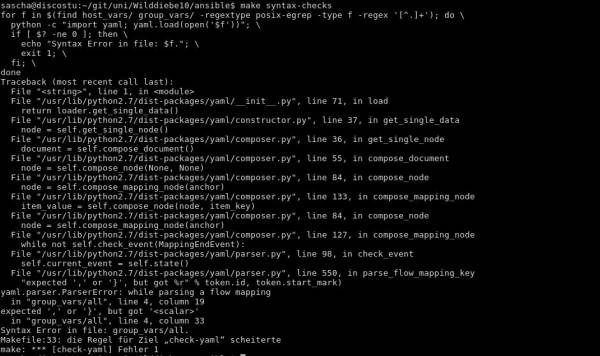
\includegraphics[scale=0.75]{images/syntaxchecks.jpg}
	\caption{Syntaxprüfung mit unserem Skript}
	\label{img:syntaxcheck}
\end{figure}

\subsubsection{Integrationstests}
Da Ansible im Moment noch keine Möglichkeit bietet den Code z.B. Unittests zu unterziehen, nutzen wir die Möglichkeit von Github Integrationstests über die Platform Travis-CI durchzuführen. Hierzu wird im Repository unter \newline  \code{ansible/tests} eine Testumgebung definiert, welche (so weit wie möglich) einem Fileserver entspricht. Hier werden alle genutzten und, zur Erfüllung der Aufgabe, benötigten Funktionen getestet. Eingeschränkt testbare Funktionen, wie z.B. der Aufbau der VPN Verbindung, werden im Rahmen der Möglichkeiten getestet. Funktionen, welche eine Netzwerkverbindung zu anderen Systemen benötigen, können auf dem Travis-CI System nicht getestet werden. Die dazugehörigen Testfälle\ref{subsec:testfaelle} werden im Repository unter \code{.travis.yml} definiert. Die Tests werden automatisch beim Hochladen eines neuen Patchsets im Git Repository durchgeführt.

\begin{figure}[!htbp]
	\centering
		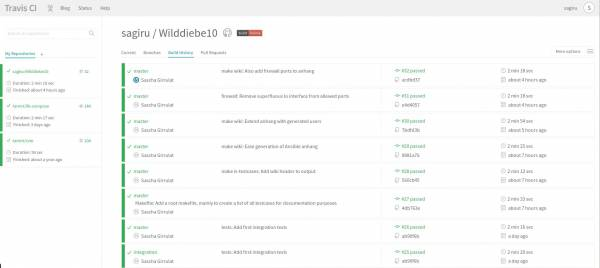
\includegraphics[scale=0.75]{images/travisci.jpg}
	\caption{Travis CI Oberfläche}
	\label{img:travisci}
\end{figure}

%----------------------------------------------------------------------------------------
%	SECTION AUSBLICK
%----------------------------------------------------------------------------------------

\section{Ausblick}
\label{sec:ausblick}
In diesem Abschnitt werden die Maßnahmen zusammengefasst, die wir als notwendig identifiziert haben, die jedoch im Rahmen des Projekte nicht umgesetzt werden konnten.

\subsection{Geplante technische Maßnahmen}
\begin{itemize}
\item Aufnahme in die Domäne mayerbrot.intern
\item Authentisierung in SAMBA gegen das AD, Fallback auf lokale Konten
\item Monitoring (Nagios\footcite{nagios}/Check\_MK)
\begin{itemize}
	\item Überwachung der von uns gewünschten aktiven Prozesse, CPU-/RAM-/HDD-Auslastung
	\item Benachrichtigung per Mail bei Warnmeldungen und Problemen
	\item Visualisierung mit NagVis
	\item Aufnahme der Monitoring-Umgebung in Sicherheits- und Betriebskonzepte
\end{itemize}
\end{itemize}

\subsection{Gewünschte organisatorische Maßnahmen}
\begin{itemize}
\item IT Sicherheitsbeauftragter
\item Vereinheitlichung der Sicherheitskonzepte zwischen den Gruppen
\item gemeinsames Betriebskonzept für alle Gruppen (siehe Betriebshandbuch)
\item klar festgelegte Risiko Owner für übernommene Risiken
\item alle Gruppen umfassende und ausführliche Auslegung des Sicherheitskonzeptes, in Vorbereitung auf eine mögliche Zertifizierung (nach welchem Standard dann auch immer\footcite{wikiCyberSecStandards})
\end{itemize}

\subsection{Blick über den Tellerrand}
\label{subsec:tellerrand}
Auch wenn sich unser Auftrag sehr konkret auf Installation und Betrieb zweier Dateiserver beschränkt, so verstehen wir unsere Aufgabe auch so, dass wir die Gesamtumgebung für die Anwender im Blick behalten sollten. Deshalb haben wir auch Vorschläge gesammelt, die über das hinaus gehen, was von uns erwartet wurde.
\begin{itemize}
\item \textbf{Active Directory / Domäne}: Im vereinigten Netz Nord/Süd existieren mindestens $2 \times 5 = 10$ Gruppen und $5 \times 5 \times 2 = 50$ Benutzerkonten jeweils für Mailserver, Webserver, CA und Dateiserver. Diese alle einzeln und händisch zu verwalten ist ein administrativer Albtraum (d.h. ineffizient, nicht nachvollziehbar, führt zu inkonsistenten Datenbeständen, usw.). Daher ist die Zusammenführung in einer Domäne zu befürworten.
\item \textbf{VoIP Umgebung} (mögliche Realisierung: Asterisk mit SIP-Clients): Zum Betrieb einer modernen IT-Lösung für Unternehmen gehört auch, sich Gedanken darüber zu machen, wie die Mitarbeiter sicher und effizient miteinander sprechen können. Darüber hinaus gibt es zahlreiche weitere Anforderungen, die nur eine professionelle Lösung abdecken kann, z.B. Callcenter (z.B. für den Benutzerservice), Telekonferenzen, Faxdienste und die Integration mobiler Telefonie.
\item Integrierte Sicherheit / \textbf{Security by Design}\footcite{waidner2013entwicklung}: erst eine aufeinander abgestimmte Client-Server-Architektur, bei der die IT-Abteilung Zugriff auf (und volle Kontrolle über) alle Systeme hat, kann ein wirksames Schutzniveau gewährleisten und die technische Lösung so gestalten, dass der Anwender das System einfach und sicher benutzen kann.
\end{itemize}
%----------------------------------------------------------------------------------------
%	SECTION FAZIT
%----------------------------------------------------------------------------------------
\newpage
\section{Fazit}
\setlength{\epigraphwidth}{.4\textwidth}
\epigraph{"`Nur Amateure greifen Maschinen an. Profis zielen auf Menschen."'}{\textit{Bruce Schneier}}

\subsection{Statement zum Praktikum}
Das Thema IT-Sicherheit ist zweifelsohne brandaktuell und übt eine große Faszination selbst auf IT-Laien aus: Vom "`Hacken"' in Hollywood-Filmen bis hin zu den zahlreichen Artikeln in Zeitungen und Zeitschriften bei aktuellen Ereignissen, steht die Relevanz des Themas nicht zur Diskussion.\\

Bei der konkreten Umsetzung des Praktikums haben wir lange über die Anforderungsspezifikation diskutiert: Ist die sehr offene und nur grob umrissene Aufgabenstellung positiv, weil sie die Studierenden zu Selbstverantwortung motiviert und uns ermöglicht, weitgehend selbst Entscheidungen zu treffen? Oder fehlt dem Projekt ein klarer Bezugspunkt: Kein Lastenheft; kein Kunde, an dessen Wünschen man sich orientieren kann und muss; keine Unternehmensleitung, welche die IT-Abteilung auf einen einheitlichen Kurs bringt. Die PMA hatten viele gute Ideen, doch das Fehlen von klaren Hierarchien bedeutet eben auch, dass viele gute Ideen nebeneinander her laufen; daraus entstehen redundante Werkzeuge und Maßnahmen und das vergeudet Ressourcen, die doch in jedem Projekt knapp bemessen sind. Andererseits ging es ja auch gerade darum, aus dem Chaos Ordnung zu erschaffen und eine eigene Organisation aufzubauen, wo vorher keine war.\\

Aus technischer Sicht haben wir im Abschnitt \ref{subsec:tellerrand} bereits einige Themen beschrieben, die für zukünftige Praktika interessant sein könnten. \\

In jedem Fall sind wir dafür dankbar, dass es dieses Praktikum gibt und dass wir in einem Land und zu einer Zeit leben, in der wir uns eingehend mit diesem Thema auseinandersetzen konnten.

\subsection{Projekterfolg}
Es ist uns in der vorgegebenen Zeit gelungen zwei Datei-Server in Betrieb zu nehmen, die für ihren sicheren Betrieb notwendigen Maßnahmen - seien sie organisatorischer oder technischer Art - umfassend zu analysieren und den größten Teil dieser Maßnahmen anschließend zu implementieren. Nach dem von uns entwickelten Maßstab\ref{subsec:si} haben wir unser Ziel zu $95\%$ erreicht. \\

Es bleibt die Frage zu beantworten, was mit den restlichen $5\%$ der Maßnahmen geschehen ist, die sich aus der Sicherheitsanalyse ergeben haben. Hardwarenahe Sicherheitsfunktionen konnten aus Kostengründen nicht realisiert werden; andere technische Verbesserungen - etwa das Monitoring - wurden aus Zeitgründen nicht realisiert. Die von uns vorgesehen organisatorischen Maßnahmen sind vollständig implementiert, insofern wir dafür nicht auf Zuarbeit anderer Gruppen angewiesen waren, von denen es leider oft keine Rückmeldung auf unsere Anfragen gab.

Dennoch: Wäre dies eine produktiv eingesetzte Umgebung, so läge ein großer Teil der Arbeit noch vor uns. Jetzt würde es darum gehen, dem Service den Feinschliff zu verpassen, in der Praxis auftretende Komplikationen zu beheben und die Absicherung iterativ zu verbessern. Da dies jedoch kein Produktivsystem ist, steht in unseren Gedanken der Lerneffekt im Vordergrund, den wir aus diesem Projekt für unser Studium mitnehmen. \\

Bei einem solch komplexen Projekt bleibt es nicht aus, dass Fehler passieren. Mancher Satz ergibt im Nachgang keinen Sinn, ein Teil der Software-Konfiguration ist lückenhaft oder kompromittiert sogar die Sicherheit. Wir machen uns keine Illusionen: Weder unser System noch unsere Vorstellung davon ist frei von Bugs. Eine Binsenweisheit lautet "`Aus Fehlern wird man klug"'. Ganz so, wie sich in der IT-Sicherheit beim Aufdecken von Schwachstellen zunächst alle darauf einigen, worum es bei dieser Lücke genau geht\footcite{wikiCVE} und anschließend gemeinsam versuchen sie zu beheben, wünschen auch wir uns, dass wir aus diesem Projekt gemeinsam lernen können die Zukunft der IT sicher zu gestalten.

%----------------------------------------------------------------------------------------
%	SECTION GLOSSAR
%----------------------------------------------------------------------------------------

\newpage
%\printglossaries

\section{Glossar}
\begin{center}
\captionof{table}{Begriffsdefinitionen im Kontext dieses Projektes}
\begin{longtable}{p{3.2cm}p{12cm}}
\toprule
Begriff & Bedeutung im Kontext dieses Projektes \\
\midrule
at Rest Verschlüsselung & Verschlüsselung von dauerhaft gespeicherten Daten \\
\midrule
CIO & Leiter der IT-Abteilung, aus dem englischen Chief Information Officer. Im Kontext dieses Projektes sind damit die Kursbetreuer gemeint. \\
\midrule
Dateiserver \newline Fileserver & Server, der einen festgelegten Bereich eines Dateisystems anderen Benutzern über das Netzwerk zur Verfügung stellt. Der Begriff ist ohne Kontext technisch unspezifisch; er bezieht sich nicht auf ein konkretes Protokoll oder eine Softwarelösung (FTP, SMB, Owncloud, etc.) \\
\midrule
Dienst & Ein im Hintergrund laufender Prozess auf einem Computer \\
\midrule
Hard Limit & Gibt den maximal nutzbaren Speicherplatz oder die maximal verwendbare Dateianzahl an. Ein Benutzer kann dieses Limit niemals überschreiten. Ein Erreichen dieses Limits ist für den Benutzer gleichzusetzen mit dem Verbrauch des verfügbaren Speicherplatzes \\
\midrule
Service & Eine für den Kunden bereitgestellte Servicedienstleistung \\
\midrule
Sicherheit \newline sicher \newline abgesichert & Ein IT Service gilt hier als sicher, wenn er die Anforderungen des BSI IT-Grundschutzes erfüllt. \\
\midrule
Soft Limit & Ist eine Begrenzung, welche kleiner oder gleich dem Hard Limit gesetzt werden muss. Wird das Soft Limit überschritten, so erhält der Benutzer den Zustand ``Over Quota''. Das Soft Limit kann bis zum Wert des Hard Limits überschritten werden \\
\midrule
Projektmitarbeiter \newline (PMA) & Studierende in den Gruppen 5 und 10 \\
\midrule
Anwendungs- \newline daten & Anwendungsspezifische Dateien, ggf. mit Anwenderbezug \\
\midrule
Systemdaten & Dateien des Betriebssystems, inklusive Einstellungen ohne Anwenderbezug \\
\midrule
Protokolldaten & Daten, die der Überwachung und Nachvollziehbarkeit von Anwendungs- oder Systemereignissen dienen \\
\midrule
Anwesenheit \newline anwesend & Als anwesend werden in diesem Projekt alle natürlichen Personen bezeichnet, die - zumindest teilweise - an einer Besprechung teilgenommen haben. Bei fernmündlichen Besprechungen (Mumble, Telekonferenz, etc.) wird als anwesend gezählt, wer am System angemeldet war. \\
\midrule
Technische \newline Dokumentation & Die technische Dokumentation umfasst alle Beschreibungen, WIE etwas in technischer Ausführung getan werden muss / getan wurde. Demgegenüber beantwortet das Betriebshandbuch die Frage, WAS getan werden muss. \\
\bottomrule
\end{longtable}
\end{center}

%----------------------------------------------------------------------------------------
%	SECTION BIBLIOGRAPHIE
%----------------------------------------------------------------------------------------

\newpage
\printbibliography

\appendix
[defaults]
roles_path = ./roles:./vendor

\section{Testprotokoll}
\captionof{table}{Identifizierte Maßnahmen}
\label{tab:massnahmen}
\begin{longtable}{p{6.8cm}p{2.4cm}p{2.4cm}p{3cm}}
\toprule
Funktion & Status Nord & Status Süd & Bemerkungen \\
\midrule
\textbf{Korrektheit und Vollständigkeit der Ansible Konfiguration }
\begin{itemize}
\item
  Server komplett zurücksetzen und Ansible Konfiguration durchführen
\item
  läuft durch ohne Fehler
\end{itemize} & OK & OK & \\
\midrule
\textbf{Einbinden Netzlaufwerk}

\begin{itemize}
\item
  Windows 8.1+ Client
\item
  AD Anmeldung
\item
  Transport via AES
\end{itemize} & OK & OK & \\
\midrule
\textbf{Daten schreiben auf Freigabe}

\begin{itemize}
\item
  Linux (Samba 4.x) Client
\end{itemize}

\begin{itemize}
\item
  Transport via AES
\end{itemize} & OK & OK & \\
\midrule
\textbf{Daten lesen von Freigabe}

\begin{itemize}
\item
  Windows 8.1+ Client
\item
  Transport via AES
\end{itemize} & OK & OK & \\
\midrule
\textbf{Einbinden Netzlaufwerk "Jeder"}

\begin{itemize}
\item
  Linux (Samba 4.x) Client
\end{itemize} & OK & OK & \\
\midrule
\textbf{Schreiben auf Jeder Freigabe }

\begin{itemize}
\item
  Windows 8.1+ Client
\item
  AD Anmeldung
\item
  Transport via AES
\end{itemize} & OK & OK & \\
\midrule
\textbf{Quotas}

\begin{itemize}
\item
  Windows 8.1+ Client
\item
  AD Anmeldung
\item
  Schreiben von \textgreater{}100 MB
\end{itemize} & OK & OK & \\
\midrule
\textbf{Quotas Jeder }

\begin{itemize}
\item
  Linux (Samba 4.x) Client
\item
  Schreiben von \textgreater{}100 MB
\end{itemize} & OK & OK & \\
\midrule
\textbf{Virus schreiben}

\begin{itemize}
\item
  EICAR-Testdatei auf Freigabe schreiben
\item 
  Eintrag von ClamAV im lokalen Log: Eicar-Test-Signature
\item 
  Eintrag im rsyslog auf anderem Server
\item
  Zugriff wird verhindert
\end{itemize} & OK & OK & \\
\midrule
\textbf{Zugriff via ipv6 nicht möglich}

\begin{itemize}
\item
  Zugriff von interner IP auf SMB Freigabe per IPv6
\item
  Zugriff von externer IP auf SMB Freigabe per IPv6
\end{itemize} & OK & OK & \\
\midrule
\textbf{Automatisches Backup}

\begin{itemize}
\item
  anlegen von Referenzdatei auf persönlicher Freigabe
\item
  anlegen von Referenzdatei auf Jeder-Freigabe
\item
  Überprüfung der Backup-Datei auf dem jeweils anderen Server nach 24h
\end{itemize} & & & \\
\midrule
\textbf{Syslog}

\begin{itemize}
\item
  Anmeldung mit Admin-Account auf Server
\item
  Ausführen von SUDO-ping
\item
  Anmeldung und ping sind im lokalen Log vorhanden
\item
  Anmeldung und ping sind im remote-log vorhanden
\end{itemize} & & & \\
\midrule
\textbf{Gesicherter Login}

\begin{itemize}
\item
  Test-Login mit Admin-Account und falschem Passwort wird nach max. 10
  Versuchen abgelehnt
\item
  Zeitpunkt des letzten Login und Logout werden beim Anmelden mitgeteilt
\end{itemize} & & & \\

\bottomrule
\end{longtable}


\end{document}
